\documentclass[a4paper,12pt]{scrartcl}

\author{Matthew Cocci}
\title{Notes to Mathematical Statistics}
\date{}
\usepackage{enumitem} %Has to do with enumeration	
\usepackage{amsfonts}
\usepackage{amsmath}
\usepackage{amsthm} %allows for labeling of theorems
\usepackage[T1]{fontenc}
\usepackage[utf8]{inputenc}
\usepackage{blindtext}
\usepackage{graphicx}
\usepackage{hyperref}
\hypersetup{
    colorlinks=true,
    linkcolor=black,
    citecolor=black,
    filecolor=black,
    urlcolor=black,
}
%\numberwithin{equation}{section} 
%, This labels the equations in relation to the sections rather than other equations
%\numberwithin{equation}{subsection} %This labels relative to subsections
\newtheorem{thm}{Theorem}[section]
\newtheorem{lem}[thm]{Lemma}
\newtheorem{prop}[thm]{Proposition}
\newtheorem{cor}[thm]{Corollary}
\setkomafont{disposition}{\normalfont\bfseries}
\usepackage{appendix}
\usepackage{subfigure} % plotting multiple figures at once




\begin{document}
\maketitle

\tableofcontents
\newpage

\paragraph{Notation} Throughout the notes, I will adhere to a few 
conventions for the sake of clarity.  In particular, capital letters
like $Y$ will typically denote \emph{random variables}, while 
lower case letters like $y$ will denote realizations of random
variables---observed data points.  Almost always, $\theta$ will be
used to denote a parameter or vector of parameters that we hope to 
estimate.


\section{Estimation of Parameters}

Most of statistics is about optimally estimating parameters using 
observed data. Specifically let's define a few terms/concepts:
\paragraph{Definition}
      An \textbf{Estimator} is a function of random variables
      that maps to a random variable for the parameter.  
      Specifically, we could describe
      an estimator as a function
	 \[ \hat{\theta}: \{Y_1, \ldots Y_n\} \rightarrow RV.\]
      For example, if take want to guess the mean height of adult women
      and we observe $n$ women, we might define the estimator:
	 $\bar{Y} =  (Y_1 + \cdots + Y_n)/n$.
      More generally, an \emph{estimator} is denoted
	 \[ \hat{\theta}(Y_1, \ldots , Y_n).\]
      \begin{itemize}
      \item[-]{
      \textbf{Note} It's important to recognize that in this context,
      $\bar{Y}$ and $\hat{\theta}(Y_1, \ldots , Y_n)$ are 
      \emph{random variables} with their own specific distributions, 
      not particular, unique values.
      }
      \end{itemize}
      
\paragraph{Definition}
      Next, we define an \textbf{estimate} to be a computed value,
      an actual number, that we get by plugging the observed data into
      the estimator function.  For example, we measured womens height
      and plug that into the above function to get
	 $\bar{y} =  (y_1 + \cdots + y_n)/n$.
      More generally, an \emph{estimate} is denoted
	 \[ \hat{\theta}(y_1, \ldots , y_n).\]
      This is a specific unique value derived from observed data.

\section{Parameter Bias}

\subsection{Definition}

It appears that we would desire our estimators to be \textbf{unbiased},
which means that
   \[ \underbrace{\int \cdots \int}_{n\; times} 
      \hat{\theta}(y_1,\ldots,y_n) \;
      f_{Y_1,\ldots,Y_n}(y_1,\ldots,y_n) \; dy_1 \ldots dy_n = \theta \]
\textbf{Note} that $\int \cdots \int$ is called the \emph{support}, 
and it ranges over the values for which the joint distribution,
$f_{Y_1,\ldots,Y_n}(\cdot)$ is positive.

\subsection{Problems}

There are reasons why the criterion of unbiasedness might not be a good
idea:
\begin{enumerate}
   \item{The estimator might be crazy.  For example, suppose that $Y$
      follows a Poisson distribution: 
	 \[ P(Y=y) = e^{-\theta} \frac{\theta^y}{\theta!}.\]
      Now suppose that we want an unbiased estimator of $e^{-2\theta}$.
      Well, it turns out that the only unbiased estimator of 
      $e^{-2\theta}$ is the function
	 \[ g(Y) = \begin{cases} +1 & \text{$y$ even} \\
	       -1 & \text{$y$ odd} \end{cases}.\]
      But this is clearly ridiculous, as $e^{-2\theta}$ will be between
      0 and 1. So those choices are nuts.
      } 
   \item{There might not be \emph{any} unbiased estimate of what you're
      trying to estimate.}
   \item{Sometimes, the mean square error of a biased estimator may be 
      less than the mean square error of \emph{any} unbiased
      estimator, where we define the mean square error to be
      \[ \underbrace{\int \cdots \int}_{\text{the support}}
	 \left( \hat{\theta}(y_1, \ldots, y_n) - \theta\right)^2
	 f_{Y_1,\ldots, Y_n}(y_1,\ldots,y_n)\; dy_1\ldots dy_n \]
      \[\qquad = Var\left[\hat{\theta}(Y_1,\ldots,Y_n)\right]
	 + [\text{Bias of } \hat{\theta}(Y_1,\ldots,Y_n)]^2 \]
      where the bias is defined to be 
      \[ \text{Bias of } \hat{\theta}(Y_1,\ldots,Y_n) = 
	 [\text{Mean of } \hat{\theta}(Y_1,\ldots,Y_n)] - \theta.\]
      So it's totally conceivable that the variance of the biased
      estimator would be very small, despite the bias.
   }
\end{enumerate}

\subsection{Conclusion}

Despite the critiques just given, asking for an unbiased is often
not so problematic.  In fact, we'll often try to find
the \emph{minimum-variance unbiased estimator}, or the MVU estimator
of a given parameter, $\theta$.  The MVU estimator is defined to be that
estimator of $\theta$ that has the smallest possible
variance of the entire class of unbiased estimators.
\\
\\
But before we go about finding them, we will have to take a detour
into the realm of order statistics, which have several nice properties
when it comes to finding the MVU estimator. 

\newpage

\section{Order Statistics}

Order Statistics are part of a larger field called 
\emph{non-parametric} statistics, or sometimes \emph{distribution-free}
statistics.


\subsection{Definitions}

Suppose that $Y_1, \ldots, Y_n$ are i.i.d RV's. From there, define
   \[ Y_{(1)} = \min\{Y_1, \ldots, Y_n\} = Y_{(\min)}  \]
   \[ Y_{(n)} = \max\{Y_1, \ldots, Y_n\} = Y_{(\max)}  \]
Similarly, if we rank-order all of them in a row, the $i$th order
statistic is the $i$th in line and is denoted $Y_{(i)}$.
\\
\\
Important to note: even though the $Y_i$ were all independent, the order
statistics $Y_{(i)}$ will \emph{not} be independent.  In fact, the
order statistics will \emph{all} have different distributions than
that of the original $Y_i$, and they will all differ from \emph{each
other} as well.

\subsection{Density Functions of Order Statistics}

Let's consider the $i$th order statistic and try to find its 
distribution, $f_{Y_{(i)}}\left(y_{(i)}\right)$. To do so, we will
want to formulate two equivalent expressions, then solve them out for
the pdf. So first,
\begin{equation}
   \label{first}
   P\left(y \leq Y_{(i)} \leq y + \delta y\right) = 
      f_{Y_{(i)}}\left(y\right)\delta y + O(\delta y)^2 
\end{equation}
Equation \ref{first} is relatively clear, once we define $O(\delta y)^2$
to be an error term of order $(\delta y)^2$.  Now for the second 
formulation, we'll recall the cdf of $Y_i$ 
\begin{equation}
   F_Y(y) = \int^t_{-\infty} f_Y(y) \; dy = P(Y \leq y) 
\end{equation}
In order for the $i$th order statistic to be in the bucket 
$[y, y+\delta y]$, you need $i-1$ observations before or at $y$,
and $n-i$ after or at $y+ \delta y$. This corresponds to the 
probability
\begin{align}
      \label{second}
      P\left(y \leq Y_{(i)} \leq y + \delta y\right) = 
      &\frac{n!}{(i-1)!1!(n-i)!}\left[\left(F_Y(y)\right)^{i-1}\right]
      \notag\\ 
      &\times\left[f_Y(y)\delta y\right]
      \left[\left(1 - F_Y(y + \delta y)\right)^{n-i}\right] + 
      O(\delta y)^2 
\end{align} 
Now that we have two equivalent expressions for the relevant probability,
we can equate Expressions \ref{first} and \ref{second}, cancel out the
errors, divide both sides by $\delta y$, then take the limit as 
$\delta y \rightarrow 0$ to get
\begin{equation}
   \label{orderpdf}
   f_{Y_{(i)}}\left(y\right) = \frac{n!}{(i-1)!(n-i)!} 
   \left[\left(F_Y(y)\right)^{i-1}\right]
   \left[f_Y(y)\right]
   \left[\left(1 - F_Y(y)\right)^{n-i}\right]
\end{equation}

\subsection{Range}

Next, a very useful Random Variable to know would be the \emph{range}
defined
   \[ R = Y_{(n)} - Y_{(1)}\]
The expectation is rather straightforward:
   \[ ER = E\left[Y_{(n)}\right] - E\left[Y_{(1)}\right].\]
The variance, however, is a little more complicated.  In order to 
compute the variance, we'll need the joint density function of 
$Y_{(1)}$ and $Y_{(n)}$. 
Using an direct generalization and extension of the method in which
we found the pdf of the $i$th order statistic, it can be show that 
\begin{align}
   f_{Y_{(i)}, Y_{(j)}}\left(u, v\right) 
   &= \frac{n!}{(i-1)!(j-i-1)!(n-j)!} 
   \left[\left(F_Y(u)\right)^{i-1}\right] f_Y(u)
   \notag \\
   &\times\left[\left(F_Y(v) - F_Y(u)\right)^{j-i-1}\right]
   f_Y(v) \left[\left(1-F_Y(v)\right)^{n-j}\right]
\end{align}
where $u = y_{(i)}$ and $v = y_{(j)}$, $i<j$.  
This simplifies considerably if we restrict ourselves to the case where
$i=1$ and $j=n$:
   \[ f_{Y_{(1)}, Y_{(n)}}\left(u, v\right) =
      n(n-1) \left[ f_y( u, v) \left( F_Y(v) - F_Y(u)\right)^{n-2}
	 f_Y(v)\right] \]
where, in this case, $u = y_{(1)}$ and $v = y_{(n)}$.  
\\
\\
From there, we can try to get at things like $Var(R)$.


\newpage


\section{The Cramer-Rao Inequality}

In general, we hope to find minimum-variance unbiased (MVU) 
estimators. One approach is the Cramer-Rao inequality approach. But
before we get there, let's go through some notation.

\subsection{Notation}

We'll be consider $n$ random variables ($Y_1, \ldots, Y_n$) which
don't necessarily have to be iid. Together, they have joint density
function 
   \[ f = f_{Y_1, \ldots, Y_n}(y_1, \ldots, y_n; \theta) \]
which depends on parameter $\theta$. Note that $f$ is just shorthand
for the expression above.
\\
\\
Second, we let $S$ represent the \emph{support} of $f$, where the 
support is the set of all values such that $f > 0$.
\\
\\
Next, we let $\tau(\theta)$ be \emph{any} arbitrary function of $\theta$
that we wish to estimate. The function $\tau(\theta)$ could be 
$\theta$, $2\theta^2$, etc. 
\\
\\
Finally, we specify a function that takes as its arguments the 
data, then returns an unbiased estimate for $\tau(\theta)$.  
This is written
   \[\hat{\tau} =  \hat{\tau}(Y_1, \ldots, Y_n) \]
where $\hat{\tau}$ represents any arbitrary \emph{unbiased} estimator of 
$\tau(\theta)$. \footnote{Note, there are possibly infinitely many of 
them.}

\subsection{Statement of the Cramer-Rao Inequality}

We now come to an important result in estimation, the Cramer-Rao 
Inequality. Note that this is a \emph{very} general result, as it does 
not assume independence
or identical distribution of the different $Y_i$ that we use to 
estimate a certain parameter.

The \emph{Cramer-Rao Inequality} states that, provided the
support $S$ does \emph{not} depend upon the parameter $\theta$, 
   \begin{equation}
      \label{cramrao}
      Var(\hat{\tau})\geq\frac{-\left[ \frac{d\tau(\theta)}{d\theta}
	 \right]^2}{
	 E\left[ \frac{d^2(\ln f)}{d\theta^2} \right]}
   \end{equation}
for any choice of $\hat{\tau}$.\footnote{The proof is given in the 
appendix.}  Now why is this useful?  Well, if we 
happen to know an unbiased estimator of $\tau(\theta)$ whose variance
equals the RHS of Equation \ref{cramrao}, then it is in fact \emph{the}
MVU estimator of $\tau(\theta)$.

\subsection{Special Cases}

{\sl Case 1}: Suppose the $Y_i$ are, in fact, iid. Then we have that
   \[ f = f_{Y_1}(y_1 ; \theta) \times \cdots f_{Y_n}(y_n ; \theta).\]
   From there, it can be show that the expectation in the denominator
   simplifies to give us a special case of the Cramer-Rao inequality:
   \begin{equation}
      \label{cramrao.sp1}
      Var(\hat{\tau})\geq\frac{-\left[ \frac{d\tau(\theta)}{d\theta}
	 \right]^2}{
	 n \cdot E\left[ \frac{d^2(\ln f_{Y_i}(y_i))}{d\theta^2} \right]}
   \end{equation}
{\sl Case 2}: Next, suppose we're trying to estimate simply the
   parameter $\theta$ so that $\tau(\theta) = \theta$. Then the
   Cramer-Rao inequality simplifies to
   \begin{equation}
      \label{cramrao.sp2}
      Var(\hat{\tau})\geq\frac{-1}{
	 E\left[ \frac{d^2(\ln f)}{d\theta^2} \right]}
   \end{equation}

\subsection{Limitations}

While useful, the Cramer-Rao Inequality may be too restrictive in some
cases. For instance,
\begin{enumerate}
   \item{We might be able to think of an unbiased estimator  
      whose variance achieves the CR bound.
      }
   \item{There might not even exist and unbiased estimator that can
      achieve the CR bound.}
   \item{The CR bound only applies if the support does \emph{not} 
      depend upon $\theta$.}
\end{enumerate}

\subsection{When is the Cramer-Rao Bound Achievable?}

A natural question to ask is ``When exactly can we hit the 
Cramer-Rao bound?'' This requires a little thought.  So first, we 
go back, to where we started in the proof to get the inequality
in the first place:
   \[ 0 \leq (Corr(W,V))^2 \leq 1.\]
When is this inequality an equality on the upper end? Well, whenever
there is perfect correlation---when one is a linear function of the
other:
   \[ V = a + bW.\]
Now that we know the conditions, recall what we took to be $W$ and
$V$ when we plugged into the above inequality to the CR inequality:
   \[ \qquad W = \hat{\tau}, \qquad V = \frac{1}{f} \frac{df}{d\theta}
      \]
Since one has to be a linear function of the other, this implies
   \[ \frac{1}{f} \frac{df}{d\theta} = A(\theta) + B(\theta) 
      \hat{\tau}(Y_1,\ldots,Y_n) \quad
      \Rightarrow \quad \ln f(\theta) = C(\theta) + D(\theta) 
      \hat{\tau}(Y_1,\ldots,Y_n) + g(y_1, \ldots, y_2)  \]
\begin{equation}
   \label{cr.form}
    \Rightarrow f(\theta) = h(y_1, \ldots, y_n) e^{C(\theta)  
      + D(\theta)  \hat{\tau}} 
   \end{equation}
where $C(\theta) = \int A(\theta) \; d\theta$ and $D(\theta) = 
\int B(\theta) \; d\theta$.
\\
\\
Now, we just need to note one more thing. Assume that the Cramer-Rao
bound is, in fact, achievable. Again, this means
   \[ \frac{1}{f} \frac{df}{d\theta} = A(\theta) + B(\theta) 
      \hat{\tau}.\]
Now let's take expectations (with respect to the random variables, not
$\theta$) throughout:
\begin{equation}
   \label{cr.exp}
    E\left[\frac{1}{f} \frac{df}{d\theta}\right] = E
      \left[A(\theta) + B(\theta) \hat{\tau}\right]
\end{equation}
On the LHS, everything simplifies to\footnote{
   Note, we could interchange the differential and the integral signs 
because $S$ does not depend upon $\theta$. Also, $k$ just stood for
some unknown constant that doesn't depend upon $\theta$.}
   \begin{align*} 
      E\left[\frac{1}{f} \frac{df}{d\theta}\right] &= 
      \int \cdots \int_S \left[\frac{1}{f} \frac{df}{d\theta}\right] f
      \; d\mathbf{y} =  
      \int \cdots \int_S \frac{df}{d\theta}
      \; d\mathbf{y} \\
      &= \frac{d}{d\theta}\left[\int \cdots \int_S f
      \; d\mathbf{y} \right]
      = \frac{d}{d\theta} \left[1 \right]\\
      &= 0
   \end{align*}
Turning to the RHS of Equation \ref{cr.exp}, we use the fact that
$\hat{\tau}$ is an \emph{unbiased} estimator of $\tau(\theta)$ to write
\begin{align*} 
     E\left[A(\theta) + B(\theta) \hat{\tau}\right] &= 
     E[ A(\theta) ] + E\left[B(\theta) \hat{\tau}(\theta)\right] \\
     &= A(\theta) + B(\theta) \tau(\theta) 
\end{align*}
Putting the LHS and RHS together and solving for $\tau(\theta)$, we get
\begin{equation}
   \label{cr.tau}
   \tau(\theta) = -\frac{A(\theta)}{B(\theta)}
\end{equation}

\newpage
\paragraph{Conclusion} If we consider everything in this 
section, we now know that \emph{if and only if} we can write the jdf
$f$ in the form of Equation 
\ref{cr.form},\footnote{And that's a big ``if''
which is by no means automatic.}
   \[ \Rightarrow f(\theta) = h(y_1, \ldots, y_n) e^{C(\theta)  
      + D(\theta)  \hat{\tau} },  \]
then the Cramer Rao bound will be achievable by \emph{some}
$\hat{\tau}$.\footnote{This also means that if $\tau(\theta)$ admits 
Cramer-Rao bound estimation, then so does any linear function of it.} 
That we can just read off of the equation just written.
But that begs the question: ``Just what $\tau(\theta)$ admits 
Cramer-Rao bound estimation?'' Well that we just also saw in equation
\ref{cr.tau}:
\[ \tau(\theta) = -\frac{A(\theta)}{B(\theta)} \]
\[ A(\theta) = \frac{d}{d\theta}\left[ C(\theta)\right] \qquad 
   B(\theta) = \frac{d}{d\theta}\left[ D(\theta)\right] \]
Finally, it can easily be show that if we assume that we can achieve
the Cramer-Rao bound with some estimator $\hat{\tau}$, then in 
the notation we used in this section
   \[ Var(\hat{\tau}) = -\frac{1}{B(\theta)} \frac{d}{d\theta} \left[
      \frac{A(\theta)}{B(\theta)}\right] \]

\paragraph{Limitations} Of course, we should consider when this
approach of identification and computation is of limited use.
\begin{enumerate}
   \item First, there might not be a way to write the jdf in the
      desired exponential form, so a function of $\theta$ might not
      exist, as we saw with the Cauchy distribution.
   \item The function of $\theta$ that we get, $\tau(\theta)$, might
      be really weird and not all that interesting in practice. So
      you find a function $\tau(\theta)$ that you \emph{can}
      find an unbiased estimator for, but that doesn't mean you want to
      or should.
\end{enumerate}


\newpage
\section{Sufficient Statistics and the Rao-Blackwell Theorem}

This is the next approach to MVU Estimation, which uses sufficient
statistics and their optimality properties. This approach is 
much more powerful than Cramer-Rao, especially because it doesn't 
require that the support be independent of $\theta$.

\subsection{Definition of Sufficient Statistics}

Suppose that we have $n$ random variables: $Y_1, \ldots, Y_n$. Together,
they have a joint density function $f_{Y_1,\dots,Y_n}(y_1, \ldots, y_n ; 
\theta).$
Then $W$ is a \emph{sufficient statistic} for $\theta$ if and only
if the conditional distribution of $Y_1, \ldots, Y_n$ given 
$W(Y_1, \ldots, Y_n)$ is independent of $\theta$. Mathematically, this
is expressed
\begin{align}
   \label{ss1}
   f_{Y_1,\dots,Y_n}(y_1, \ldots, y_n | w; \theta) &= 
   f_{Y_1,\dots,Y_n}(y_1, \ldots, y_n | w) \notag\\
   \Leftrightarrow \quad
   \frac{f_{Y_1,\dots,Y_n, W}(y_1, \ldots, y_n,  w; \theta)}{
	  f_{W}(w; \theta) } &= 
      f_{Y_1,\dots,Y_n}(y_1, \ldots, y_n | w)
\end{align}
Note that often when we compute the numerator in Equation \ref{ss1},
the $W$ term will give you no additional information 
over and above the $Y_1, \ldots, Y_n$ individually.  In that case,
the numerator reduces the problem to checking that
\begin{equation}
   \label{ss3}
   \frac{f_{Y_1,\dots,Y_n}(y_1, \ldots, y_n; \theta)}{f_W(w;\theta)}
      =f_{Y_1,\dots,Y_n}(y_1, \ldots, y_n | w)
\end{equation}
If it turns out that the conditional distribution of 

\subsection{Properties and Intuition}

{\sl Vector Sufficient Statistics}:
Note that we can generalize so that a sufficient statistic is a vector,
such as $(W_1, W_2, \ldots, W_k)$. 
\\
\\
{\sl Uniqueness}: Sufficient statistics aren't 
necessarily unique. For example, suppose $W_1$ is a sufficient statistic.
Then the vector $(W_1, W_2)$ will be too for any choice of $W_2$
since $W_1$ is sufficient on its own. Also, it's immediately clear that
the vectors $(Y_1, \ldots, Y_n)$ and $(Y_{(1)}, \ldots, Y_{(n)})$ will
also be sufficient statistics since they encapsulate all of the data
trivially.
\\
\\
{\sl Intuition}:
Suppose there are two people, some data ($y_1, \ldots, y_n)$, and
some function of the data $W=W(Y_1, \ldots, Y_n)$. Now suppose that
I give Person 1 all of the $n$ data points. Next suppose I give
Person 2 just $W(y_1, \ldots, y_n)$. If the information I gave 
Person 1 \emph{equals} the information I gave Person 2 from 
the standpoint of information about $\theta$, then $W$ is a sufficient
statistic for $\theta$.


\subsection{Rao-Blackwell Theorem, Part 1}

Suppose that a sufficient statistic, $W$, for $\theta$ exists.  Let
$\tau(\theta)$ be any function of $\theta$ admitting unbiased
estimation, i.e. for which an unbiased estimator, $\hat{\tau}$, of
$\tau(\theta)$ exists. Then a \emph{unique}, \emph{minimum variance}
unbiased estimator of $\tau(\theta)$ is some function of $W$. 
\\
\\
So if we find a sufficient statistic, $W$, and can fiddle around to get 
some function of $W$ that does in fact have an expectation of $\theta$,
thank the gods of statistics, because you just found \emph{the}
unique MVU estimator of $\theta$.
\\
\\
{\sl Improvement over Cramer-Rao}: The Rao-Blackwell Theorem 
allows us to estimate parameters $\tau'(\theta)$ that are \emph{not}
linear functions of whatever $\tau(\theta)$ that the Cramer-Rao approach
indicates admits CR bound estimation. It's much
more general. Moreover, it works \emph{whether or not} the support
depends upon $\theta$.


\subsection{Minimal, Non-Trivial Sufficient Statistics (MNTSS)}

We have a few requirements for finding really good, powerful 
sufficient statistics.
\begin{enumerate}
   \item We want them to be \emph{minimal}, in that we compress 
      information as
      much as possible. So if both $W_1$ and $(W_1, W_2)$ are sufficient
      statistics, don't use the latter. It doesn't compress information
      enough and is non-minimal.
   \item We want our sufficient statistics to be non-trivial. So 
      the vector $(W_1, \ldots, W_k)$ should be such that 
      $k < n$ so we achieve \emph{some} compression.
\end{enumerate}
Note that all of this implies that any \emph{scalar} SS must be 
non-minimal and non-trivial. 
\\
\\
We want to know whether, in any given situation, a scalar MNTSS
exists, and, if there is one, how can we find it? To do so, there
are two situations we must consider separately:
\begin{itemize}
   \item[-] The support $S$ does \emph{not} depend upon $\theta$.
   \item[-] The support $S$ \emph{does} depend upon $\theta$.
\end{itemize}
Both situations unfortunately require very different approaches, so
we'll handle each in turn.

\newpage
\subsection{Finding a MNTSS, $S$ Independent of $\theta$}

Here, we document three cases to find an MNTSS whenever $S$ is 
independent of $\theta$: the Factorization
approach, the Smith-Jones approach, and the Exponential Family 
approach.

\subsubsection{Factorization Approach}

$W$ is a scalar SS for $\theta$ if and only if 
\begin{align}
   \label{factor}
   \frac{f_{Y_1,\dots,Y_n}(y_1, \ldots, y_n; \theta)}{
      f_W(w; \theta)} &= k(y_1,\ldots,y_n)  
      \notag\\
   \Rightarrow f_{Y_1,\dots,Y_n}(y_1, \ldots, y_n; \theta) &= 
      k(y_1,\ldots,y_n) f_W(w; \theta)
\end{align}
where $k(y_1, \ldots, y_n)$ is some constant function of the data
that is independent of $\theta$ and where $f_W(w; \theta)$ is
some function of $\theta$ and the sufficient statistic, $W$, only.

\subsubsection{Smith-Jones Approach}

Again, we hope to find a scalar sufficient statistic, which would
automatically be a MNTSS. Now suppose we have two statisticians, 
Smith and Jones. 
\begin{center}
\begin{tabular}{ l | l}
   Person & Has observed values for $Y_1, \ldots, Y_n$ of \\ \hline 
   Smith & $y_{11}, y_{12}, \ldots, y_{1n}$ \\
   Jones & $y_{21}, y_{22}, \ldots, y_{2n}$ 
\end{tabular}
\end{center}
Next we define the ratio $R$ as the ratio of the probability of 
Smith's data to that of Jones' data:
   \[ R = \frac{f(y_{11}, y_{12}, \ldots, y_{1n}; \theta)}{ f(
      y_{21}, y_{22}, \ldots, y_{2n}; \theta)}\]
Then the necessary and sufficient condition that the function
$g(Y_1, \ldots, Y_n)$ be a scalar sufficient statistic for $\theta$
is that that the ratio $R$ is independent of $\theta$ 
\emph{if and only if}
   \[ g(Y_{11}, Y_{12}, \ldots, Y_{1n})
      =  g(Y_{21}, Y_{22}, \ldots, Y_{2n}) \]
In practice, this means that we form the ratio, $R$. Then we try to
find the function $g(Y_1,\ldots, Y_n)$ such that $R$ has no
$\theta$ term in it whenever the sufficient statistics match for 
both Smith and Jones.\footnote{
This follows from the factorization
approach. Because see by Equation \ref{factor} that if we form 
the ratio of the two likelihoods, the $f_W(w;\theta)$ will cancel 
out, removing all occurrences of $\theta$ with it, provided 
   \[ g(Y_{11}, Y_{12}, \ldots, Y_{1n})
      =  g(Y_{21}, Y_{22}, \ldots, Y_{2n}). \]
All that will be left is a ratio of two constants that come from 
the data.}
\\
\\
{\sl Generalization to $\theta$ as a Vector}: Suppose 
$\theta = (\theta_1, \ldots, \theta_k)$. Form $R$ as above. 
Now suppose that $g_i(Y_1,  \ldots, Y_n)$ for $i=1, \ldots, s$
are $s$ linearly independent functions of $Y_1, \ldots, Y_n$. 
Then the necessary and sufficient condition that the vector 
\begin{equation}
\label{sj}
 \begin{pmatrix} g_1(Y_1, \ldots, Y_n) & g_2(Y_1, \ldots, Y_n) & \ldots
      & g_s(Y_1, \ldots, Y_n) \end{pmatrix}
\end{equation}
is a non-trivial sufficient statistic for $\theta$ is that $s<n$
and also that $R$ is independent of $\theta$ \emph{if an only if} 
the following $s$ conditions hold:
\begin{equation}
   \label{sj2}
   g_i(Y_{11}, \ldots, Y_{1n}) =  g_i(Y_{21}, \ldots, Y_{2n}), 
      \qquad i = 1, \ldots,s 
\end{equation}
Now that we have a non-trivial sufficient statistic, we can ask ``Is
it minimal?'' To that question, the vector in expression \ref{sj} is 
minimal if there does not exist another vector of length $t<s$ 
such that $R$ is independent of $\theta$ if and only if the 
analogous conditions in Equations \ref{sj2} hold for the new vector.
   


\subsubsection{Exponential Family Approach}

Suppose that the jdf can be written as\footnote{This should look
familiar to the Cramer-Rao approach.}
   \[ f_{Y_1, \ldots, Y_n}(y_1, \ldots, y_n; \theta)=h(y_1, \ldots, y_n)
      e^{C(\theta) + D(\theta) \hat{\theta}}.\]
Then $\hat{\theta}$ is a scalar, sufficient statistic for $\theta$.
\\
\\
{\sl Generalization to $\theta$ as a Vector}: Suppose we can write the
jdf (in abbreviated vector notation) as
\[ f_{\mathbf{Y}}(\mathbf{y}; \Theta)
      = h(\mathbf{y})\cdot
      \exp\left\{ {C(\Theta) + \sum^s_{j=1} 
      D_j(\Theta) g_j(\mathbf{y}) }\right\}, \qquad s < n
	 \]
\[ \mathbf{Y} = (Y_1, \ldots, Y_n), \qquad 
   \mathbf{y} = (y_1, \ldots, y_n),
   \qquad \Theta = (\theta_1, \ldots, \theta_k) \]
where the functions $D_1, \ldots, D_s$ are linearly independent functions
of $\Theta$. Then 
\[ \begin{pmatrix} g_1(Y_1, \ldots, Y_n) & g_2(Y_1, \ldots, Y_n) & \ldots
      & g_s(Y_1, \ldots, Y_n) \end{pmatrix} \]
is a MNTSS for $\Theta = (\theta_1, \ldots, \theta_k)$.


\newpage
\subsection{Finding a MNTSS, $S$ Dependent Upon $\theta$}

In this case, we will only consider cases where $Y_1, \ldots, Y_n$
are iid due to the complex nature of the relationship between 
$S$ and $\theta$.


\paragraph{Support of the Form $[a, b(\theta)]$}
Suppose that $f_Y(y; \theta)$ factorizes into 
   \[ f_Y(y; \theta) = g(y) h(\theta).\]
Then $Y_{(n)}$ is a MNTSS for $\theta$. Intuitively, if you know
that $Y_{(n)}$ is the largest value of your observations, nothing
else tells you \emph{anything} extra about the upper bound, $b(\theta)$.
Rao-Blackwell then ensures that your resulting estimator from the
MNTSS is unique, provided it is unbiased.

\paragraph{Support of the form $[a(\theta), b(\theta)]$} For 
this case, we deal with two concrete examples:
\begin{enumerate}
   \item Suppose $f_Y(y) = 1$ and 
      $\theta < y < \theta +1$, then your MNTSS is going to be the 
      vector
	 \[ \begin{pmatrix} Y_{(1)} & Y_{(n)} \end{pmatrix}.\]
      Note, this is interesting because you're trying to estimate 
      \emph{one} parameter, but your MNTSS is a \emph{two}-dimensional 
      vector.
   \item Next, suppose that $f_Y(y) = 1/2\theta$ and that
      $-\theta < y < \theta$. Then the MNTSS will be 
	 \[ \max\{ -Y_{(1)}, Y_{(n)}\} \]
\end{enumerate}

\subsection{Full Rao-Blackwell Theorem}

The full theorem has two parts. We already saw part 1, but we'll it
repeat here for completeness. So 
suppose we want to estimate $\tau(\theta)$
and some sufficient statistic, which we denote $W$, 
exists for $\theta$. Then
\begin{enumerate}
   \item The unique MVU estimator of $\tau(\theta)$ is some function 
      of $W$.
   \item Let $\hat{\tau} = \hat{\tau}(Y_1, \ldots, Y_n)$ be \emph{any}
      unbiased estimator of $\tau(\theta)$. Then the \emph{unique}
      MVU estimator of $\tau(\theta)$ is guaranteed (!) to be
	 \[ E\left[\hat{\tau}(Y_1, \ldots, Y_n) | W \right] \] 
      That's really powerful and pretty awesome.
\end{enumerate}
{\sl Applying the Rao-Blackwell Theorem}: The two different components
give us two different approaches to find a unique MVU estimate. Here
they are numbered by the part of the RB Theorem to which they apply:
\begin{enumerate}
   \item Find the SS. Manipulate and fiddle 
      until you get some $\hat{\tau}$ such that $E[\hat{\tau}] = 
      \tau(\theta)$. 
   \item Find \emph{any} old unbiased estimator 
      $\hat{\tau}$. And it could be crazy!\footnote{See the appendix
      for one example.} Like one you'd 
      \emph{never} think of using to estimate $\tau(\theta)$ in 
      a million years. But just so long as its expectation is 
      $\tau(\theta)$, RB Part 2 tells you it will work 
      (and what to do!).
\end{enumerate}

\subsection{Potential Problems}

As always, no method is perfect, and there are a few issues with 
the sufficient statistic and Rao-Blackwell approach to finding 
MVU estimators:
\begin{enumerate}
   \item There might not \emph{be} an MNTSS to search for.
   \item We have to find an unbiased estimator of $\tau(\theta)$ if
      we want to use Rao-Blackwell, Part 2. However, there might
      not \emph{be} such an unbiased estimator.
   \item Even if there is an unbiased estimator of $\tau(\theta)$,
      we might not be smart enough to find it.
\end{enumerate}




%%%%%%
\newpage

\section{Maximum Likelihood Estimation}

Broadly speaking, maximum likelihood approach is a practical approach
that overcomes the difficulties associated with sufficient 
statistics---the very same difficulties we outlined above. It is also
an improvement over the method of moments, which was popular in
statistics prior to MLE methods.

\subsection{Finding Maximum Likelihood Estimators}

Our main goal will be to find maximum likelihood estimators: functions
of random variables that can be use to estimate certain parameters.
So to start, suppose we have $n$ random variables (not necessarily
iid) with some jdf:
\begin{equation}
   \label{mlejdf}
    f_{Y_1, \ldots, Y_n}(y_1, \ldots, y_n; \theta) 
\end{equation}
which is dependent upon some fixed, but unknown parameter, $\theta$.
\\
\\
Now comes the big insight: turn that logic around. Rather than think
of the jdf as a function of $y_1, \ldots, y_n$ with $\theta$ fixed,
assume the $y_1, \ldots, y_n$ are fixed and $\theta$ is a variable
in what we rename the \emph{likelihood function}. 
This will have the same functional form as the jdf in Equation
\ref{mlejdf}, but we change our idea of what's fixed. This gives us
\begin{equation}
   \label{mlelik}
    L(\theta; y_1, \ldots, y_n) \quad\Rightarrow \quad
    \hat{\theta}_{\text{MLE}} =  
   \arg \max_\theta L(\theta; y_1, \ldots, y_n) 
\end{equation}
Note, that while this works, we'll often apply the same method to
the \emph{log} of the likelihood function, which turns the product
in the jdf into a sum. This is often more algebraically and 
computationally tractable, so we often solve
\[ \hat{\theta}_{\text{MLE}}  =
   \arg \max_\theta \ell(\theta; y_1, \ldots, y_n), 
   \qquad \ell = \ln L(\theta; y_1, \ldots, y_n)  \]
Often, we'll find the maximum likelihood estimator by taking the 
derivative, setting the result equal to zero, and solving for the
parameter. However, sometimes we'll have a \emph{boundary maximum},
most often when the support depends upon the parameter.\footnote{
Note that MLEs aren't guaranteed to biased at all. But often they will
be, and when they aren't they're usually pretty close and do
well enough.}
\\
\\
{\sl Multiparameter Case}: Finally, we can generalize to 
allow for multiple parameters:
   \[ f_{Y_1, \ldots Y_n}(y_1, \ldots, y_n; \theta_1, \ldots, \theta_k)
      \Rightarrow
      L(\theta_1, \ldots, \theta_k; y_1, \ldots, y_n )
      \]
nn which case, we take partial derivatives, set them equal to zero, 
and solve for $\theta_1, \ldots, \theta_k$.
\\
\\
{\sl Constraints}: In the multiparameter case particularly, we will
sometimes want to allow for constraints, which can be easily
implemented by a Lagrange multiplier technique when we do the
maximization.


\newpage
\subsection{Properties of Maximum Likelihood Estimators}

Maximum likelihood estimators have some very nice properties, which
is why we like to use them in the first place.\footnote{When I use
the shorthand ``MLE,'' I'm
explicitly talking about maximum likelihood estimat\textbf{ors},
which are functions of random variables, and more general that
estimat\textbf{es}, which are simply numbers computed from the data.}
Let's review those properties now:
\begin{enumerate}
   \item {\sl Invariance Property}: Suppose that $\tau = \tau(\theta)$
      is a monotonically increasing or decreasing function of 
      $\theta$. Then
      \[ \hat{\tau}_{\text{MLE}} = \tau\left(\theta_{\text{MLE}}\right)
	 \]
      where $\hat{\tau}_{\text{MLE}}$ is the MLE for $\tau(\theta)$
      and $\theta_{\text{MLE}}$ is the MLE for $\theta$.
   \item {\sl Relation to MNTSS's}: If a scalar MNTSS exists,
      then it is a function of the maximum likelihood estimator.

      \begin{proof} Here's an informal sketch. We know by the 
	 factorization criterion that the jdf, and hence the likelihood,
	 will look like
	    \[ f = L = g(y_1, \ldots, y_n) h(\hat{\theta}_\text{MNTSS},
	       \theta) \]
	 where $g$ is independent of $\theta$.
	 Well, to max L with respect to $\theta$, we will be maxing
	 $h$ with respect to $\theta$, which implies that $\theta$
	 is some function of the MNTSS. 
      \end{proof}
   \item {\sl Optimality Properties of MLEs}: If we let $\tau(\theta)$
      be any function of $\theta$ and let $\hat{\tau}_{\text{MLE}}$
      be the maximum likelihood estimator of $\tau(\theta)$, then
      under the regularity conditions assumed in the Cramer-Rao
      bound section, 
	 \[ \lim_{n\rightarrow \infty} E[\hat{\tau}_{\text{MLE}}] 
	 = \tau(\theta) \]
	 \[ \lim_{n\rightarrow \infty}
	    \frac{ Var(\hat{\tau}_{\text{MLE}})}{\text{Cramer-Rao
	    bound for $\tau(\theta)$}} \rightarrow 1 \]
      while the distribution of $\hat{\tau}_{\text{MLE}}$ approaches
      the normal distribution as $n\rightarrow \infty$. This is really
      powerful stuff. So in words, what this means is
      \begin{enumerate}
	 \item Asymptotically unbiased.
	 \item Asymptotically normal.
	 \item Asymptotically has variance approaching the CR bound.
      \end{enumerate}
\end{enumerate}

\newpage
\subsection{Application: Simple Linear Regression}

Simple linear regression provides a great testing ground to apply
some of the techniques described above. So let's assume we have $n$
random variables $Y_i$ that are \emph{independently}, but 
\emph{not} identically distributed as follows
   \[ Y_i \sim N(\alpha + \beta x_i,\; \sigma^2) \]
If we form the likelihood and solve for our three unknowns, we get
MLEs of 
\[ \hat{\beta} = \frac{\sum Y_i (x_i - \bar{x})}{\sum (x_i-\bar{x})^2},
   \qquad \hat{\alpha}=\bar{Y} - \hat{\beta} \bar{x}, \qquad
   \hat{\sigma}^2 = \frac{\sum (Y_i - \hat{\alpha}-\hat{\beta}x_i)^2}{
   n}
   \]
Our estimators of $\alpha$ and $\beta$ are both unbiased; however,
the estimator of $\sigma^2$ is biased a bit.
\\
\\
{\sl Strategy in Selecting Covariates}: We know that our estimator
of $\beta$ is unbiased, but what about the variance of $\hat{\beta}$?
It's not hard to see from the formula for $\hat{\beta}$ that, since
the $x_i$ terms are known constants,
   \[ Var(\hat{\beta}) = \frac{\sigma^2}{\sum (x_i - \bar{x})^2} \]
This suggests that to \emph{minimize} the variance of our estimator, we
want to \emph{maximize} the variance of our covariates.\footnote{  
However, we shouldn't do this blindly by clustering our observations
at two extreme $x_i$ values. This wouldn't allow us to see
whether the relationship was linear, quadratic, or some other higher
order relationship. Therefore, we should have values along the 
spectrum of possible $x_i$ values, but we should, at the same time,
try to make that spectrum of possible values as wide as we can.}



\newpage
\section{Transformation Theory}

Throughout this section, we'll only consider continuous random 
variables. So let's start with $n$ random variables, $X_1, \ldots,
X_n$, (not necessarily iid) which have jdf
   \[ f_{X_1, \ldots, X_n}(x_1, \ldots, x_n) \]
Now let's suppose that we have $Y$, which is some function 
   \[ Y = g(X_1, \ldots, X_n) \]
Let's review some reasons why we might want to find such a function,
$Y$:
\begin{enumerate}
   \item Often, an MLE---call it $Y$---will be a function of the
      $X_i$. To know the properties of $Y$, we have to know it's
      distribution.
   \item Many test statistics are, in fact, \emph{derived} statistics
      with parameters dependent on the variables $X_i$.
\end{enumerate}

\subsection{Univariate Case, Monotonic}

Throughout, we'll assume that $X$ has a known density function, 
$f_X(x)$. If we define $Y = g(X)$, we want to find $f_Y(y)$.
\\
\\
{\sl Monotonically Increasing/Decreasing}: We can group these two
cases together to get two equivalent formulations,
\begin{align*}
   f_Y(y) &= \left[f_X(x) \left\lvert \frac{dx}{dy}\right\rvert
      \right]_{x = g^{-1}(y)} \\
      &= \left[ f_X(x) / \left\lvert \frac{dy}{dx}\right\rvert
      \right]_{x = g^{-1}(y)}
\end{align*}


\subsection{Univariate Case, Non-Monotonic}

Suppose that we have some RV, $X$, with distribution $f_X(x)$. 
We now want the distribution for $Y=g(X)$, where $g$ is some 
non-monotonic function of $X$. Then
\begin{equation}
   \label{nonmontrans}
   f_Y(y) = \sum_i \left[ f_X(x_i) \left\lvert \frac{dx_i}{dy}
      \right\rvert \right]_{x_i=g_i^{-1}(y)} 
\end{equation}
where each $g_i^{-1}(y)$ is a different functional inverse of $y$.
Note that the range of $i$ in the sum can vary depending upon 
how non-monotonic the function is and how many functional inverses
exist.\footnote{Non-monotonic transformations allow for discontinuous
probability density functions.}

\subsection{Multivariate Case}

Suppose that we have $X_1, \ldots, X_n$ with jdf $f_{X_1, \ldots, X_n}(
x_1, \ldots, x_n)$. Now let 
\begin{align*}
   Y_1 &= Y_1(X_1, \ldots, X_n) \\
   Y_2 &= Y_2(X_1, \ldots, X_n)\\
   \vdots &= \qquad \vdots\\
   Y_n &= Y_n(X_1, \ldots, X_n)
\end{align*}
We assume that the functions are 1-to-1, akin to the monotonicity
assumption in the univariate case. Now we want to know the 
jdf, $f_{Y_1, \ldots, Y_n}(y_1, \ldots, y_n)$. This we compute
\begin{align*}
   f_{Y_1, \ldots, Y_n}(y_1, \ldots, y_n) &= \left[
      f_{X_1, \ldots, X_n}(x_1, \ldots, x_n) \lvert J \rvert 
      \right]_{X_i}
      \qquad X_i = X_i(Y_1, \ldots, Y_n)\\
   &= \left[
      f_{X_1, \ldots, X_n}(x_1, \ldots, x_n)\frac{1}{\lvert J^*\rvert}
      \right]_{X_i}
\end{align*}
where the $J$ and $J^*$ terms are the determinants of the Jacobian
matrices
\begin{equation}
   J = \begin{bmatrix} \frac{\partial x_1}{\partial y_1} &
      \frac{\partial x_1}{\partial y_2} & \cdots & 
      \frac{\partial x_1}{\partial y_n} \\
      \vdots & & \ddots & \vdots \\
      \frac{\partial x_n}{\partial y_1} & 
      \frac{\partial x_n}{\partial y_2} & \cdots &
      \frac{\partial x_n}{\partial y_n}  
   \end{bmatrix} \qquad \qquad
   J^* = \begin{bmatrix} \frac{\partial y_1}{\partial x_1} &
      \frac{\partial y_1}{\partial x_2} & \cdots & 
      \frac{\partial y_1}{\partial x_n} \\
      \vdots & & \ddots & \vdots \\
      \frac{\partial y_n}{\partial x_1} & 
      \frac{\partial y_n}{\partial x_2} & \cdots &
      \frac{\partial y_n}{\partial x_n}  
   \end{bmatrix}
\end{equation}
Often, we will even use this to do transformations that are not
1-to-1. That will involve doing a transformation that \emph{is}
1-to-1 using this method with dummy variables, then integrating
out those dummy variables.




\newpage
\subsection{Applications of Univariate Case}

\subsubsection{Simulations via Uniform Distribution}

Suppose we want to draw from a distribution, $f_X(x)$ for the variable
$X$. Now let's consider the random variable, where we suppose
the integral has an analytical solution:
\begin{equation}
   \label{unifMC}
   Y = \int^x_a f_X(t) \; dt = h(X) 
\end{equation}
We can apply our transformation rule to get the distribution of $Y$:
\begin{align*}
    f_Y(y) &= \left[ f_X(x) / \left\lvert\frac{dy}{dx} \right\rvert
       \right] =\left[ f_X(x) / \frac{d}{dx} \left( \int^x_a 
	  f_X(t)\; dt\right) \right] \\
      &=\left[ f_X(x) / f_X(x) \right]  = 1
\end{align*}
In other words, the density function of $Y$ is the \emph{uniform
distribution}. This means that we can draw from a uniform 
distribution, compute the integral in Equation \ref{unifMC}, invert,
and set
   \[ Y = h^{-1}(Y) \]
in order to obtain a draw from $X$. This allows us to draw from
any arbitrary distribution, so long as we can compute the integral
in Equation \ref{unifMC} and invert the resulting function.



\subsubsection{Square of a Normal Random Variable}

Suppose the $X\sim$ NID(0,1), and $Y = X^2$. Clearly, we're in 
the non-monotonic case, so let's find the distribution of $Y$ with
that in mind:
\begin{align*}
   f_Y(y) &= \frac{1}{\sqrt{2\pi}} \left[ e^{-\frac{1}{2}x_1^2}/
      \left\lvert \frac{dy}{dx_1}\right\rvert \right]_{x_1 = \sqrt{y}} +
      \frac{1}{\sqrt{2\pi}} \left[ e^{-\frac{1}{2}x_1^2}/
      \left\lvert \frac{dy}{dx_2}\right\rvert \right]_{x_2 =-\sqrt{y}}\\
   &= \frac{2}{\sqrt{2\pi}} \left[ e^{-\frac{1}{2} y} / 2\sqrt{y}
      \right ] \\
   &= \frac{1}{\sqrt{2\pi}} y^{-\frac{1}{2}} e^{-\frac{1}{2} y}
\end{align*}
which is a $\chi^2_1$ distribution.\footnote{Of course, you have
to be able to simulate a normal random variable to simulate a 
$\chi^2_1$ random variable, and that's a bit tricky. But we'll do 
that below.} 


\newpage
\subsection{Applications of Multivariate Case}

In this case, we'll have to use Jacobian matrices and also dummy
variables to generate random variables and compute the distributions
for derived statistics.


\subsubsection{Generating a N(0,1) Random Variable}

We can't actually generate a \emph{single} N(0,1) RV, but we can
generate two and throw one out, so let's do that. Assume
$X_1, X_2\sim \text{NID}(0,1)$:
   \[ f_{X_1, X_2}(x_1,x_2) = \frac{1}{2\pi} e^{-\frac{1}{2}(x_1^2 +
      x_2^2)} \]
Now to do our change of variables, let's define 
\begin{align*}
   X_1 &= R \cos\theta, \qquad R > 0 \\
   X_2 &= R \sin \theta, \qquad \theta \in [0,2\pi)
\end{align*}
If we take $R = Y_1$ and $\theta = Y_2$, then we form the Jacobian:
\begin{align}
   J &= \det \begin{bmatrix} \frac{\partial X_1}{\partial R} &
   \frac{\partial X_1}{\partial \theta} \\\\
   \frac{\partial X_2}{\partial R} &
   \frac{\partial X_2}{\partial \theta} 
   \end{bmatrix} = 
   \det \begin{bmatrix} \cos \theta & -R \sin \theta \\
      \sin \theta & R \cos \theta \end{bmatrix} \notag\\
   &= R(\cos^2 \theta + \sin^2 \theta) = R
\end{align}
Now, applying the multivariate transformation above, we get
our joint density and distribution functions under the transformed 
variables: 
   \[f_{R,\theta}(r,\theta) = \frac{1}{2\pi} r e^{-\frac{1}{2}r^2}\]
   \[ F_R(r) = \int^R_0 \int^{2\pi}_0 \frac{1}{2\pi} r e^{-\frac{1}{2}
      r^2} \; d\theta\;dr = 1 - e^{-\frac{1}{2} R^2} \]
   \[ F_\theta(\theta) = 
      \int^\theta_0 \int^\infty_0 \frac{1}{2\pi} r e^{-\frac{1}{2}
   r^2} \;dr\; d\theta = \frac{\theta}{2\pi}
      \]
To get normal random variables, we draw $U_1$ and $U_2$ from the
Uniform(0,1) distribution, set 
   \[ U_1 = 1- e^{-\frac{1}{2}R^2} \quad \Rightarrow \quad 
      R = \sqrt{-2\ln(1-U_1)} \]
   \[ U_2 = \frac{\theta}{2\pi} \quad \Rightarrow \quad 
      \theta = 2\pi U_2 \]
   \[ X_1 = \sqrt{-2\ln(1-U_1)} \cos (2\pi U_2), \qquad 
      X_2 = \sqrt{-2\ln(1-U_1)} \sin (2\pi U_2) \]
Which is how you generate two standard normal random variables.


\subsubsection{Student's t-Distribution}

In order to generate a variable that has $t$ distribution with 
$n-1$ degrees of freedom,
we start by supposing that $Y_i\sim \text{NID}(\mu,\sigma^2)$. From
there, we define
\begin{align*}
   \bar{Y} = \frac{1}{n} \sum^n_{i=1} Y_i \qquad 
   S^2 &= \frac{1}{n-1} \sum^n_{i=1} (Y_i - \bar{Y})^2 \\
   &=\frac{1}{n-1} \left( Y_1^2 + \cdots + Y_n^2 - n \bar{Y}^2\right)
\end{align*}
The statistics $\bar{Y}$ and $S^2$ are useful because they are both
unbiased estimators of $\mu$ and $\sigma^2$, respectively. 
And before we get to the derivation, we make one final note: 
\emph{Cochran's Theorem}
says that $\bar{Y}$ and $S^2$ are independent for the normal 
distribution.\footnote{This holds for \emph{no} other distributions;
it is unique to the normal.} 
\\
\\
Now let's define the statistic, $T$,
whose distribution we hope to find:
   \[ T = \frac{\bar{Y}-\mu}{S/\sqrt{n}} \qquad Y_i \sim \text{NID}(\mu,
      \sigma^2) \]
But after a bit of rearranging and variable definitions, we get
\begin{align*}
   T &= \frac{(\bar{Y}-\mu)\sqrt{n} }{S} = \frac{
      \frac{\bar{Y}-\mu}{\sigma/\sqrt{n}}}{\sqrt{\frac{S^2}{\sigma^2}
      \cdot \frac{n-1}{n-1}}} \\
      &= \frac{W_1}{\sqrt{W_2 / (n-1)}}
\end{align*}
Now it's clear by how we defined $W_1$ and $W_2$ that $W_1$ has a
N(0,1) distribution, while $W_2$ has a $\chi^2$ distribution with
$n-1$ degrees of freedom. Since $W_1$ and $W_2$ are \emph{independent}
by Cochran's theorem, the jdf of $W_1, W_2$ is 
   \[ f_{W_1, W_2}(w_1, w_2) = \left(
      \frac{1}{\sqrt{2\pi}} \; e^{-\frac{1}{2} w_1^2}\right)\left( 
      \frac{1}{ 2^{\frac{n-1}{2}} \Gamma\left(\frac{n-1}{2}\right)}
      \; w_2^{\frac{n-1}{2} -1} e^{-\frac{1}{2}
      w_2}\right)
      \]
Now we just hope to find the jdf of $T$. Since transformations must be
1-to-1 in the number of variables, we'll choose
a dummy variable, $V$, and define to simplify the mess of fractions
in the jdf:
\[ V =W_2, \qquad k = \frac{1}{\sqrt{2\pi}} \cdot \frac{1}{
   2^{\frac{n-1}{2}} \Gamma\left(\frac{n-1}{2}\right)} \]
This leads us to from the Jacobian matrix to go from $W_1$ and
$W_2$ to $T$ and $V$:
\[ J^* = \det \begin{bmatrix} \frac{\partial T}{\partial W_1} &
   \frac{\partial T}{\partial W_2} \\
   \frac{\partial V}{\partial W_1} &
   \frac{\partial V}{\partial W_2} \end{bmatrix} = 
   \begin{vmatrix} \frac{1}{\sqrt{W_2/(n-1)}} && \frac{\partial T}{
      \partial W_2} \\ 0 && 1 
   \end{vmatrix} = \frac{1}{\sqrt{W_2/(n-1)}}
   \]
Now we can get the jdf of $T$ and $V$:
\begin{align*}
   f_{T,V}(t,v) &= \left[ f_{W_1,W_2}(w_1, w_2) \cdot
      \lvert J^* \rvert^{-1}
      \right]^{w_1 = g_1^{-1}(t,v)}_{w_2 = g_2^{-1}(t,v)}\\
   &= \left[ k \cdot e^{-\frac{1}{2} w_1^2} 
      w_2^{\frac{n-1}{2} - 1} e^{-\frac{1}{2} w_2}  \left(
      \frac{1}{\sqrt{w_2/(n-1)}}\right)^{-1}
      \right]^{w_1 = t \sqrt{\frac{v}{
      n-1}}}_{w_2=v}\\
      &= \frac{k}{\sqrt{n-1}} v^{\frac{n-1}{2} - \frac{1}{2}}
      e^{-\frac{1}{2} v\left( 1 + \frac{t^2}{n-1}\right)} 
\end{align*}
Now we just need to integrate out the dummy variable, $V$, to 
get the distribution of $T$, which will require some substitution:
\[ y = \frac{1}{2} v \left( 1 + \frac{t^2}{n-1} \right), \qquad
   dv = \frac{2}{\left( 1 + \frac{t^2}{n-1} \right)} \; dy \]
\begin{align*}
   \Rightarrow f_{T}(t) &=\frac{k}{\sqrt{n-1}} \int^\infty_0
      v^{\frac{n-1}{2} - \frac{1}{2}}
      e^{-\frac{1}{2} v\left( 1 + \frac{t^2}{n-1}\right)} \; dv \\
      &= \frac{k}{\sqrt{n-1}} \left( \frac{2}{ 1 + \frac{t^2}{n-1} } 
      \right)^{\frac{n-1}{2} + \frac{1}{2}} \int^\infty_0 
      y^{\frac{n-1}{2} - \frac{1}{2}} e^{-y} \; dy
\end{align*}
Now we recognize the integral as the $\Gamma(n/2)$ function, so 
we can substitute that in and substitute in for $k$ to get
\begin{align*}
   \Rightarrow f_{T}(t) &=\frac{\Gamma(n/2)}{   
      \Gamma\left(\frac{n-1}{2}\right)\sqrt{\pi(n-1)}} 
      \left( 1 + \frac{t^2}{n-1}\right)^{-\frac{n}{2}}
\end{align*}
So for a given $n$, this is the $t$-distribution with $n-1$ degrees
of freedom. 
\\
\\
Equivalently, we can also express the distribution in an equally
common formulation, where the statistic has $\nu$ degrees of freedom:
\begin{align*}
   \Rightarrow f_{T}(t) &=\frac{\Gamma\left(\frac{\nu+1}{2}\right)}{   
      \Gamma\left(\frac{\nu}{2}\right)\sqrt{\nu\pi}} 
      \left( 1 + \frac{t^2}{\nu}\right)^{-\frac{\nu+1}{2}}
\end{align*}


\newpage
\subsubsection{F-Statistic and Distribution}

Closely related to the $t$-distribution (and just as important),
we now want to find the distribution of the $F$ statistic, defined as
\[ F = \frac{ X_a / a}{X_b / b},\qquad\qquad X_a \sim \chi^2_a, \quad
   X_b \sim \chi^2_b \]
Since $X_a$ and $X_b$ are assumed independent, 
we can form the jdf as the product of the two density functions
\begin{align*}
   f_{X_a, X_b}(x_a, x_b) &= \left(\frac{1}{2^{a/2} \Gamma(a/2)}
      \; x_a^{a/2 -1} e^{-x_a/2 }\right) \left(
      \frac{1}{2^{b/2}  \Gamma(b/2)} \;
      x_b^{b/2 -1} e^{- x_b /2} \right)\\
   &= k \; x_a^{a/2 -1} \; x_b^{b/2 -1} e^{-\frac{1}{2}(x_a + x_b)} \\
   \text{where } \quad k &= \frac{1}{ 2^{\frac{a+b}{2}} \Gamma(a/2) 
      \Gamma(b/2)}
\end{align*}
Now we want to find the jdf of $F$ and our chosen dummy variable,
$G=X_b$. To do so, we start with the inverse functions and 
then form the Jacobian matrix:
   \[ X_a = \frac{a FG}{b}, \qquad X_b = G, \quad\Rightarrow \quad
     |J| = \begin{vmatrix} \frac{\partial X_a}{\partial F} &
      \frac{\partial X_a}{\partial G} \\ 
      \frac{\partial X_b}{\partial F} &
      \frac{\partial X_b}{\partial G} \end{vmatrix} =
      \begin{vmatrix}
	 \frac{a G}{b} & \frac{a F}{b} \\ 0 & 1 
      \end{vmatrix} 
      = \frac{a}{b} G
      \]
This allows us to write the trnasformed jdf 
\begin{align*}
   p_{F,G}(f,g) &= \left[ 
      k x_a^{a/2 -1} x_b^{b/2 -1} e^{-\frac{1}{2}(x_a + x_b)} 
      \left( \frac{a}{b} g\right) \right]^{x_a = a f g/b}_{x_b = g}\\
   &= k' f^{a/2 -1} g^{\frac{a+b}{2}-1} e^{-\frac{g}{2}\left(
      \frac{a}{b}f +1 \right)} \\
   \text{ Where} \qquad k' &= \frac{1}{ 2^{\frac{a+b}{2}} \Gamma(a/2) 
      \Gamma(b/2)} \left( \frac{a}{b}\right)^{\frac{a}{2}} 
\end{align*}
To get the density function of $F$, we integrate out the dummy
variable, $G=X_b$, which is a simple $\chi^2$ variable whose support
is the positive real line:
\begin{align*}
   p_F(f) &= k' f^{a/2 -1} \int^\infty_0 
      g^{\frac{a+b}{2}-1} e^{-\frac{g}{2}\left(
      \frac{a}{b}f +1 \right)} \; dg
\end{align*}
We'll make the substitution 
   \[ u = \frac{g}{2}\left(\frac{a}{b} f +1\right) , \qquad
      g = 2u \left( \frac{a}{b} f +1\right)^{-1} \]
   \[ dg = 2 \left( \frac{a}{b} f +1\right)^{-1} \; du
      \]
\begin{align*}
   \Rightarrow \qquad p_F(f) &= k' f^{a/2 -1}  \left[ 
      2 \left( \frac{a}{b} f +1\right)^{-1}\right]^{\frac{a+b}{2}}
     \int^\infty_0 u^{\frac{a+b}{2} - 1}
     e^{-u} \; du
\end{align*}
Finally, 
we recognize that the integral is simply the $\Gamma( (a+b)/2)$ 
function. This allows us to simplify $p_F$ and substitute back for
$k'$ to get
\begin{align*}
   p_F(f) &= k' f^{a/2 -1}  \left[ 
      2 \left( \frac{a}{b} f +1\right)^{-1}\right]^{\frac{a+b}{2}}
      \Gamma\left(\frac{a+b}{2}\right) \\
   \Rightarrow \qquad
   p_F(f) &= \frac{\Gamma\left(\frac{a+b}{2}\right)}{ \Gamma(a/2) 
      \Gamma(b/2)} \left( \frac{a}{b}\right)^{\frac{a}{2}} 
      f^{\frac{a}{2} -1} \left[ 
	 1 + \frac{a}{b} f \right]^{-\frac{a+b}{2}}
\end{align*}
which is the density function for $F$.


\newpage

\section{Hypothesis Testing}

There are two main approaches to \emph{hypothesis testing}: the
{\sl Classical Approach} and the {\sl Bayesian Approach}.
This section will focus exclusively on the classical approach. To do
so, we introduce a table that will be of use in our discussion that
documents the types of outcomes we might observe in hypothesis testing:
\begin{center}
   \begin{tabular}{r c}
      $\quad\qquad$ & $\qquad$ {\sl What We Claim}\\
   \end{tabular}
   \\
   \begin{tabular}{l | c c}
      {\sl True Situation} & $H_0$ True & $H_0$ False \\\hline
      $H_0$ True & \checkmark & \textbf{Type I Error}\\
      $H_0$ False & \textbf{Type II Error} & \checkmark
   \end{tabular}
\end{center}
Our hypothesis testing will invariably require us to collect 
\emph{data}, which we explicitly define as observed 
values, or realizations, of random variables; therefore,
randomness is built into the decision.


\subsection{Five Basic Steps}

In the classical approach to hypothesis testing, there are five
main steps which we will summarize here:
\begin{enumerate}
   \item Set up a null hypothesis, denoted $H_0$, \emph{explicitly}.
      Also, set up an explicit alternative hypothesis, denoted
      $H_1$. There are two forms a hypothesis, either null or 
      alternative, can take:
      \begin{itemize}
	 \item[-] {\sl Simple}: All parameters are specified 
	    numerically. For example 
	    \[ H_0: \beta = 0, \qquad H_1:\theta = 0.6\]
	 \item[-] {\sl Composite}: Not all parameters are specified
	    numerically. Examples include:
	    \begin{align*}
	       \text{One-Sided Composite } \qquad& \theta > 0.5,
	       \qquad \theta < 0.5\\
	       \text{Two-Sided Composite } \qquad& \theta \neq 0.5
	    \end{align*}
      \end{itemize}
   \item We next adopt our Type I error rate. 
      on the basis of observed data,  which equals the
      $\alpha$ level. Just to be explicit:
	 \[ \alpha = P(\text{Type I error}) \]
   \item Next, we decide on the \emph{test-statistic} that we 
      will compute in order to decide whether to accept or reject
      $H_0$ depending upon the resulting numerical value. Ideally, 
      this test statistic will be chosen based on some 
      ``optimality properties'' which we will consider below.
   \item Next, we establish the \emph{critical region} within
      which we will reject the null in favor of the alternative
      hypothesis. 
   \item Finally, we will collect data, calculate the value of the
      test statistic, and accept or reject the null based on
      whether the value of the test statistic falls within some
      critical region.
\end{enumerate}

\subsection{Using p-values}

{\sl Definition}: You can alternatively conduct Hypothesis Tests using 
p-values. A p-value is the probability of getting the 
\emph{actually observed} value (given the data) of the test 
statistic---or a value more extreme than the observed value---when
$H_0$ is true. We accept or reject using the rule
\[ \text{p-value} \leq P(\text{Type I error}) \quad 
   \Rightarrow \quad \text{Reject $H_0$} \]
Note that when working with p-values, the alternative hypothesis
specification is Duncan Hines irrelevant. You work only with the
values specified in the null.\footnote{Note that this process doesn't
really take into account model uncertainty.}


\subsection{Power}

Our Type I error is fixed at whatever value of $\alpha$ that we
chose in Step 2. But given that value of $\alpha$, we would like
to know the \emph{power} of the test, defined as
\begin{align*}
   \text{Power} &= P(\text{Reject $H_0$} | H_0 \text{ False}) 
   =1 - P(\text{Type II Error})
\end{align*}
In the case where $H_1$ is \emph{simple}, the
power is a number, but if $H_1$ is \emph{composite}, there is 
no unique value for the power.  Rather, we will have a 
\emph{power curve}
or \emph{power surface}. So suppose without loss
of generality, that the \emph{true} value of the parameter, $\theta^*$,
is greater than the \emph{null} value, $\theta_0$. 
In that case the power curve
will look something like the following.
Notice that the probability of rejection increases as 
$\theta^*-\theta_0$ increases:
\begin{figure}[h!]
   \centering
   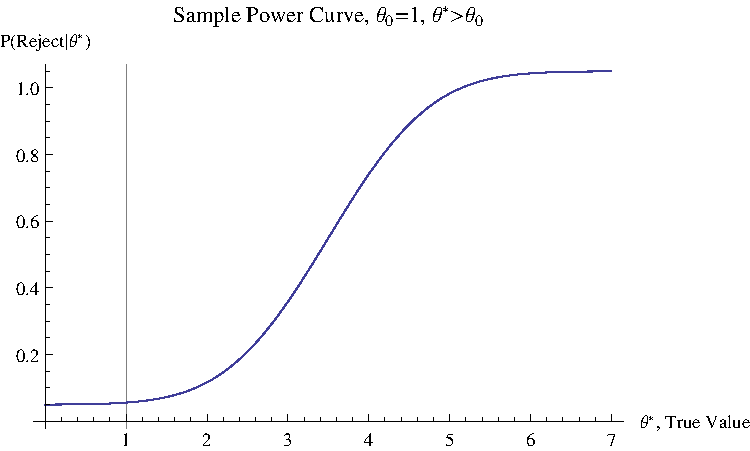
\includegraphics[scale=0.7]{SamplePowerCurve.pdf}
\end{figure}

\subsection{Neyman-Pearson Lemma}

{\sl Simple $H_0$, Simple $H_1$}: We first consider the case where 
both the null and alternative are simple, and we denote the jdfs
implied by $H_0$ and $H_1$ as $f_0$ and $f_1$, respectively. We
then form the \emph{likelihood ratio}:
\[ \text{LR} = \frac{f_0(y_1, \ldots, y_n)}{f_1(y_1, \ldots, y_n)}=
   \frac{P(\text{data under $H_0$})}{P(\text{data under $H_1$})}
   \]
The Neyman-Pearson Lemma states that the uniformly most powerful
test of $H_0$ versus $H_1$ rejects $H_0$ whenever LR $\leq K$,
where $K$ is ``sufficiently small'' given the chosen value of $\alpha$.
And by ``uniformly most powerful,'' we mean that this test 
maximizes the power (i.e. is \emph{optimal})
after controlling for the Type I error---i.e.
after setting the Type I error rate to $\alpha$.
\\
\\
{\sl Connection to Sufficient Statistics}: If a sufficient statistic, 
$W$, exists for the parameter, $\theta$, that's being tested, then 
$W$ \emph{will} be the test statistic in the hypothesis test. This 
follows from the fact that we can factorize the jdf into two
components: a function of the data only and a function of the sufficient
statistic and $\theta$.

\subsection{Applications of the Neyman-Pearson Lemma}

\subsubsection{Normal Data}

Suppose that $Y_i \sim$ NID($\mu, \sigma^2$). Furthermore, consider 
the null and alternative hypothesis
   \[ H_0: \mu = \mu_0, \qquad H_1: \mu = \mu_1, \qquad \mu_1 > \mu_0 \]
The Neyman-Pearson Lemma instructs us to form the Likelihood Ratio
\begin{align*}
   \text{LR} &= \frac{ \left(\frac{1}{\sigma \sqrt{2\pi}}\right)^n
      e^{-\frac{1}{2\sigma^2} \sum (y_i - \mu_0)^2}}{
      \left(\frac{1}{\sigma \sqrt{2\pi}}\right)^n
      e^{-\frac{1}{2\sigma^2} \sum (y_i - \mu_1)^2}}\\
   &= \exp\left\{\frac{1}{\sigma^2}(\mu_0 - \mu_1) \sum^n_{i=1} y_i - 
	 \frac{n}{2\sigma^2}\left(
      \mu_0 - \mu_1\right)\right\}
\end{align*}
Neyman-Pearson then 
tells us to reject $H_0$ when LR is sufficiently small
($\leq K$), which happens when $\sum y_i$ is sufficiently large 
($\geq K'$). Clearly, $\sum y_i$ is our test-statistic.
\\
\\
Next, we want to choose $K'$ so that the Type I error rate equals
$\alpha$:
\begin{align*}
   0.05 &= P(\Sigma\; Y_i \geq K' | \text{ $H_0$ true}) \\
   &= P\left( \frac{ \Sigma \; Y_i - n \mu_0}{\sqrt{n\sigma^2}}
      \geq \frac{K' - \mu_0}{\sqrt{n\sigma^2}} \; \rvert 
      \text{ $H_0$ true}\right) \\
   &= P\left( Z \geq \frac{K' - \mu_0}{\sqrt{n\sigma^2}} \; \rvert 
      \text{ $H_0$ true}\right) \\
   \Rightarrow Z = 1.645 &= \frac{K' - \mu_0}{\sqrt{n\sigma^2}} \\
   K' &= n\mu_0 + 1.645 \sqrt{n\sigma^2}
\end{align*}
So we have the value of $K'$ and, therefore, the critical region.

\newpage
\subsubsection{Binomial Data}

Here, we suppose that 

\newpage
\subsection{Lambda Ratio Test}

\subsubsection{Justification and Intuition}

Recall that the Neyman-Pearson lemma stated that the method gave
the uniformly most powerful tests. However, recall that power\footnote{
Unlimited power!} is defined as
   \[ \text{Power} = P(\text{Reject $H_0$} | \text{$H_1$ true}) \]
Moreover the likelihood Ratio procedure required a specification 
of the probability of the data under the alternative, $H_1$. BUT,
and here's the rub, is you're working with a \emph{composite} 
alternative, where not all parameters are specified
\begin{enumerate}
   \item Power is not a single number, but a range of values 
      depending upon the values in $H_1$, which can vary.
   \item The probability of the data under the alternative \emph{also}
      takes on a range of values.
\end{enumerate}
How to cope?
\\
\\
Well, if you wanted to know who had the best Hockey players---the US
or Canada---it's not very efficient to have all teams consisting of 
all hockey players compete against each other. So you take the 
all-stars, and have the best of the US play against the best Canadian
players.  We'll essentially do the same here.

\subsubsection{Procedure}

So suppose the null and alternative hypothesis are composite. 
We now form the Lambda Ratio by taking
\[ \lambda =    
   \frac{\max P(\text{data under $H_0$})}{
      \max P(\text{data under $H_1$})}
   \]
To find the maximum probabilities under $H_0$ and $H_1$, we
will have to differentiate the likelihood---or equivalently, the
log-likelihoods---with respect to any unspecified parameters, set
the first order conditions equal to zero, and solve. 
\\
\\
After we have the solutions, we plug back into the $\lambda$ formula 
and use the same criterion:
reject $H_0$ whenever $\lambda\leq K$,
where $K$ is ``sufficiently small'' given the chosen value of $\alpha$.
This maximizes the power after controlling for the Type I error---i.e.
after setting the value of the Type I error equal to $\alpha$.


\newpage
\subsection{Applications of the $\lambda$-Ratio Test}

\subsubsection{Normal Data, Test of the Mean}

Suppose our data is such that $Y_i \sim $NID$(\mu,\sigma^2)$, and 
we want to test the hypotheses that
   \[ H_0: \mu = \mu_0, \qquad H_1: \mu \neq \mu_0, \qquad 
      \text{$\sigma^2$ unspecified for both} \]
Note that the procedure is very much the same for the one-sided
tests. So let's carry out the $\lambda$-ratio test.
\\
\\
{\sl Max Under Null}: We maximize the log-likelihood under the null
for $\sigma^2$:
\begin{align*}
   P(\text{data} | H_0) &= \left(\frac{1}{\sigma\sqrt{2\pi}}\right)^n
      e^{-\frac{1}{2\sigma^2} \sum (y_i - \mu_0)^2 } \\
   \ln P(\text{data} | H_0) &= - n \ln \sqrt{2\pi}
      -\frac{n}{2} \ln \sigma^2 - \frac{1}{2\sigma^2}
      \sum_{i=1}^n (y_i - \mu_0)^2 \\
   \text{Solve} \Rightarrow \quad 0= 
      \frac{\partial \ln P(\text{data}}{\partial 
      \sigma^2} &= -\frac{n}{2\sigma^2} + \frac{1}{2\sigma^4} 
      \sum_{i=1}^n (y_i - \mu_0)^2 \\
   \hat{\sigma}^2_0 &= \frac{\sum (y_i - \mu_0)^2}{n}\\
   \Rightarrow\quad \max P(\text{data} | H_0) &= 
      \left(\frac{1}{\hat{\sigma}_0 \sqrt{2\pi}} \right)^n 
	 e^{-n/2}
\end{align*}
{\sl Max Under Null}: We maximize the log-likelihood under the 
alternative and solve for \emph{both} $\sigma^2$ and $\mu$ (some steps
omitted):
\begin{align*}
   P(\text{data} | H_1) &= \left(\frac{1}{\sigma\sqrt{2\pi}}\right)^n
      e^{-\frac{1}{2\sigma^2} \sum (y_i - \mu)^2 } \\
   \ln P(\text{data} | H_0) &= - n \ln \sqrt{2\pi}
      -\frac{n}{2} \ln \sigma^2 - \frac{1}{2\sigma^2}
      \sum_{i=1}^n (y_i - \mu)^2 \\
   \hat{\mu}_1 &= \bar{y}\\
   \hat{\sigma}^2_1 &= \frac{1}{n} \sum^n_{i=1} (y_i - \bar{y})^2\\
   \Rightarrow \quad \max P(\text{data} | H_1) &= 
      \left(\frac{1}{\hat{\sigma}_1 \sqrt{2\pi}} \right)^n
      e^{-n/2}
\end{align*}
\newpage
{\sl Form the $\lambda$ Ratio:} Recall, we'll want to reject if
$\lambda$ is sufficient small. So let's form the ratio using 
everything above and rearrange:
\begin{align*}
   \lambda &= \frac{\max P(\text{data under $H_0$})}{
      \max P(\text{data under $H_1$})} = \left(
      \frac{\hat{\sigma}_1^2}{\hat{\sigma}_0^2}\right)^{n/2}\\
   &= \left( \frac{\sum (y_i - \bar{y})^2}{\sum (y_i - \mu_0)^2}
      \right)^{n/2}
   = \left( \frac{\sum (y_i - \bar{y})^2}{\sum (y_i - \bar{y})^2 +
   n(\bar{y} - \mu_0)^2}
      \right)^{n/2}\\
   &= \left( \frac{1}{1 + \frac{n(\bar{y} - \mu_0)^2}{
      \sum (y_i - \bar{y})^2 }}
      \right)^{n/2}\\
   &= \left( \frac{1}{1 + \frac{t^2}{n-1}}
   \right)^{n/2} \qquad \text{where } 
   t = \frac{(\bar{y}-\mu_0)}{s/\sqrt{n}}\qquad 
   \text{and } s^2 = \frac{\sum^n_{i=1} (y_i - \bar{y})^2}{n-1} \\
\end{align*}
So you reject the null if $\lambda$ is sufficiently small, which
is equivalent to $t$ being sufficient large, implying that $t$ is you
test statistic. How large must $t$ be? Well check the distribution.

\newpage
\subsubsection{Normal Data, Test of Two Means (One-Way ANOVA, Special
   Case)}

Now suppose that we have two subsets of data with different means
but equal variance, where both sets of data are independent of each
other:
   \[ Y_{11}, \ldots, Y_{1n_1} \sim \text{NID}(\mu_1, \sigma^2) \]
   \[ Y_{21}, \ldots, Y_{2n_1} \sim \text{NID}(\mu_2, \sigma^2) \]
We want to test the following hypothesis:
\begin{align*}
   H_0:& \mu_1 = \mu_2 = \mu, \qquad \mu, \sigma^2 
      \text{ unspecified} \\
    H_1:& \mu_1, \mu_2, \sigma^2 \qquad \text{ all unspecified} 
\end{align*}
Note that $H_1$ specifies a 3D parameter space, while $H_0$ restricts
to a specific subset---a plane in parameter space.
\\
\\
{\sl Max Under Null}: We maximize the log-likelihood under the null
for $\sigma^2$ and $\mu$, since both are left unspecified.
I'll state the probabilities, then jump right to
the MLE's, which follow from some ommited, but straightforward, 
calculations:
\begin{align*}
   \arg \max_{\sigma^2, \mu} 
   P(\text{data} | H_0) &= \left( \prod^{n_1}_{i=1} \frac{1}{\sigma
      \sqrt{2\pi}} e^{-\frac{1}{2\sigma^2} (y_{1i} - \mu)^2} 
      \right) \left( \prod^{n_2}_{i=1} \frac{1}{\sigma
	 \sqrt{2\pi}} e^{-\frac{1}{2\sigma^2} (y_{2i} - \mu)^2} 
      \right)\\
   \hat{\mu} = \bar{\bar{y}}&= 
      \frac{n_1 \bar{y}_1 + n_2 \bar{y}_2}{n_1 + n_2}\\
   \hat{\sigma}^2 = \hat{\sigma}^2_0 &= \frac{1}{n_1 + n_2} 
   \left[ \sum_{i=1}^{n_1} (y_{1i} - \bar{\bar{y}})^2 + 
	 \sum_{j=1}^{n_2} (y_{2j} - \bar{\bar{y}})^2 \right]\\
   \Rightarrow \max P(\text{data} | H_0) &=
      \left( \frac{1}{\hat{\sigma}_0 \sqrt{2\pi}}\right)^{n_1+n_2}
      e^{-\frac{1}{2} (n_1+n_2)}
\end{align*}
{\sl Max Under Null}: We maximize the log-likelihood under the 
alternative for $\mu_1$, $\mu_2$, and$\sigma^2$. Again, I'll state the 
probabilities, then jump right to
the MLE's, which follow from some ommited, but straightforward, 
calculations:
\begin{align*}
   \arg \max_{\sigma^2, \mu_1,\mu_2} 
   P(\text{data} | H_1) &= \left( \prod^{n_1}_{i=1} \frac{1}{\sigma
      \sqrt{2\pi}} e^{-\frac{1}{2\sigma^2} (y_{1i} - \mu_1)^2} 
      \right) \left( \prod^{n_2}_{i=1} \frac{1}{\sigma
	 \sqrt{2\pi}} e^{-\frac{1}{2\sigma^2} (y_{2i} - \mu_2)^2} 
      \right)\\
   \mu_1 &= \bar{y}_1, \qquad \mu_2 = \bar{y}_2\\
      \hat{\sigma}^2_1 &= \frac{1}{n_1+n_2} \left[
      \sum^{n_1}_{i=1} (y_{1i} - \bar{y}_1)^2 +
      \sum^{n_2}_{j=1} (y_{2j} - \bar{y}_2)^2\right]\\
   \Rightarrow \quad \max P(\text{data} | H_1) &= 
      \left( \frac{1}{\hat{\sigma}^2_1\sqrt{2\pi}} \right)^{n_1+n_2}
      e^{-\frac{1}{2}(n_1+n_2)}
\end{align*}
\newpage
{\sl Form the $\lambda$ Ratio:} Recall, we'll want to reject if
$\lambda$ is sufficient small. So let's form the ratio using 
everything above, rewrite, and rearrange,\footnote{We'll use an 
identity to break up the denominator.}
\begin{align*}
   \lambda &= \left(\frac{\hat{\sigma}^2_1}{\hat{\sigma}^2_0}
      \right)^{\frac{n_1+n_2}{2}} = \left( \frac{ 
      \sum^{n_1}_{i=1} (y_{1i} - \bar{y}_1)^2 +
      \sum^{n_2}_{j=1} (y_{2j} - \bar{y}_2)^2}{
      \sum_{i=1}^{n_1} (y_{1i} - \bar{\bar{y}})^2 + 
      \sum_{j=1}^{n_2} (y_{2j} - \bar{\bar{y}})^2 }
      \right)^{\frac{n_1+n_2}{2}}\\
      &= \left( \frac{ 
      \sum^{n_1}_{i=1} (y_{1i} - \bar{y}_1)^2 +
      \sum^{n_2}_{j=1} (y_{2j} - \bar{y}_2)^2}{
      \sum_{i=1}^{n_1} (y_{1i} - \bar{y}_1)^2 + 
      \sum_{j=1}^{n_2} (y_{2j} - \bar{y}_2)^2 + \frac{n_1n_2}{n_1+n_2}
      (\bar{y}_1 - \bar{y}_2)^2}
      \right)^{\frac{n_1+n_2}{2}}\\
      &= \left( \frac{1}{
	 1+ \frac{n_1n_2}{n_1+n_2}\frac{(\bar{y}_1 - \bar{y}_2)^2}{ 
	 \sum (y_{1i} - \bar{y}_1)^2 +
	 \sum (y_{2j} - \bar{y}_2)^2}}
	 \right)^{\frac{n_1+n_2}{2}}\\
      &= \left( \frac{1}{
	 1+ \frac{t^2}{n_1+n_2-2}}\right)^{\frac{n_1+n_2}{2}}
	 \qquad t = \frac{\bar{y}_1 - \bar{y}_2}{s/\sqrt{\frac{n_1n_2}{
	 n_1+n_2}}} \qquad s^2 = \frac{\sum (y_{1i}-\bar{y}_1)^2
	 + \sum (y_{2j} - \bar{y})^2}{n_1+n_2-2}
\end{align*}
So that if the null is true, then $t$ has a distribution with $n+m-2$
degrees of freedom.

\paragraph{Note} This is a special case of \emph{One-Way ANOVA}, which
we cover in the next section, where $k=2$.  In this special case,
we also have the following relationship between test statistics:
   \[ F = t^2 \]

\newpage
\subsubsection{One-Way ANOVA}

Suppose we have $k$ groups of random variables. We'll be
conductiong a test of
\emph{means} (not variance, despite the name) for those $k$ groups
of the form
\[ Y_{i1}, Y_{i2}, \ldots, Y_{in_i} \qquad \text{NID}(\mu_i, \sigma^2),
      \qquad i=1, \ldots, k \]
where $\sigma^2$ is common to all groups.\footnote{It's really important
that we recognize the assumption in One-Way ANOVA that the data comes 
from \emph{normal} distributions. If we're not comfortable with that
assumption, then we will be in error if we
use the test.} Now suppose we want to test
the hypotheses
\begin{align*}
   H_0: \mu_1& = \mu_2 = \cdots = \mu_k = \mu \qquad 
      \text{ $\mu$, $\sigma^2$ unspecified} \\
   H_1: \mu_1,& \mu_2, \ldots, \mu_k, \sigma^2 \text{ all unspecified}
\end{align*}
If we carry out the normal $\lambda$ ratio procedures (maximizing 
under the null and alternative hypotheses), then we will be able to 
form the ratio and derive
\begin{align*}
   \lambda &= \left[ \frac{ \sum (y_{1i} - \bar{y}_1)^2 + \cdots +
      \sum (y_{ki} - \bar{y}_k)^2}{
      \sum (y_{1i} - \bar{\bar{y}})^2 + \cdots +
      \sum (y_{ki} - \bar{\bar{y}})^2}\right]^{\sum_{i=1}^k n_i/2}\\
   &= \left[ \frac{ \sum (y_{1i} - \bar{y}_1)^2 + \cdots +
      \sum (y_{ki} - \bar{y}_k)^2}{
      \sum (y_{1i} - \bar{y}_1)^2 + \cdots +
      \sum (y_{ki} - \bar{y}_k)^2
      + n_1(\bar{y}_1 - \bar{\bar{y}})^2 + \cdots 
      + n_k(\bar{y}_k - \bar{\bar{y}})^2
      }\right]^{\sum_{i=1}^k n_i/2}\\
   &= \left[ \frac{1}{1+ \frac{k-1}{N-1}} F\right]^{\sum_{i=1}^k n_i/2}
   \qquad F = \frac{ [n_1(\bar{y}_1 - \bar{\bar{y}})^2 + \cdots 
      + n_k(\bar{y}_k - \bar{\bar{y}})^2]/(k-1)}{
      \left[\sum (y_{1i} - \bar{y}_1)^2 + \cdots +
      \sum (y_{ki} - \bar{y}_k)^2\right]/(N-k)}
\end{align*}
So that the test statistic follows an $F$ distribution. Note that
we can also rewrite $F$ and get an alternative formulation:
\begin{align}
    F &= \frac{\text{BGSS}}{\text{WGSS}} \cdot
      \frac{N-k}{k-1} = 
      \frac{ [n_1(\bar{y}_1 - \bar{\bar{y}})^2 + \cdots 
      + n_k(\bar{y}_k - \bar{\bar{y}})^2]}{
      \left[\sum (y_{1i} - \bar{y}_1)^2 + \cdots +
      \sum (y_{ki} - \bar{y}_k)^2\right]} \cdot 
      \frac{N-k}{k-1} \label{decomp}\\
   &= \frac{ \text{BGSS}/\sigma^2}{
      \text{WGSS}/\sigma^2} \cdot 
      \frac{N-k}{k-1} \label{anovachi}
   \end{align}
From there, it can be show that if $H_0$ is true, then
\begin{itemize}
   \item[-] The numerator and denominator in 
      Equation \ref{anovachi} are independent.\footnote{Here,
      numerator and denominator refore to the left-hand fraction.
      Same for the next statement.}
   \item[-] The numerator and denominator in Equaiton 
      \ref{anovachi} are $\chi^2$ distribution
      with $k-1$ and $N-k$ degrees of freedom, respectively. This
      means that we can properly use the $F$ statistic.
   \item[-] We can think of Equations \ref{decomp} and \ref{anovachi}
      as creating ratios of signal to noise.
\end{itemize}
Therefore, ANOVA consists of breaking up the total sum of squares
into a Between Group Sum of Squares and Within Group Sum of Squares:
\[ \text{Total SS} = \sum (y_{1i}-\bar{\bar{y}})^2 + \cdots + 
   (y_{ki}-\bar{\bar{y}})^2
   = \text{BGSS} + \text{WGSS} \]


\newpage
\subsubsection{Regression}

Suppose we are studying the effect of a known treatment of some 
variable, $x_i$, on the some random response value, $Y_i$.
Further, we assume that the $Y_i$ have distribution
   \[ Y_i \sim \text{N}(\alpha + \beta x_i,\; \sigma^2) \]
Now we want to test the hypothesis that 
   \[ H_0: \beta = 0, \qquad H_1: \beta \neq 0 \]
We know the drill. We'll have to form a lambda ratio, so we need to
\begin{itemize}
   \item[-] {\sl Maximize Under $H_0$}: We have the following
      \begin{align*}
	 P(\text{data} | H_0) &= \prod^n_{i=1} \frac{1}{
	    \sigma\sqrt{2\pi}} e^{-\frac{1}{2\sigma^2} 
	    (y_i - \alpha)^2} \\
	    \Rightarrow \quad \hat{\alpha} &= \bar{y} \qquad
	    \hat{\sigma}^2_0 = \frac{\sum (y_i - \bar{y})^2}{n}\\
	 \max P(\text{data} | H_0) &= \left(\frac{1}{\sqrt{2\pi}}
	    \right)^n \left(\frac{1}{\hat{\sigma}_0^2}\right)^{n/2}
	    e^{-n/2}
      \end{align*}
   \item[-] {\sl Maximize Under $H_1$}: We have the following
      \begin{align*}
	 P(\text{data} | H_1) &= \prod^n_{i=1} \frac{1}{
	    \sigma\sqrt{2\pi}} e^{-\frac{1}{2\sigma^2} 
	    (y_i - \alpha - \beta x_i)^2} \\
	 \Rightarrow \hat{\beta} = \frac{\sum y_i(x_i - \bar{x})}{
	    \sum (x_i - \bar{x})^2} \qquad \hat{\alpha} &= \bar{y}-
	    \hat{\beta} \bar{x} \qquad \hat{\sigma}^2_1 = 
	    \frac{\sum(y_i - \hat{\alpha} - \hat{\beta}x_i)^2}{n}\\
	 \max P(\text{data} | H_1) &= \left(\frac{1}{\sqrt{2\pi}}
	    \right)^n \left(\frac{1}{\hat{\sigma}_1^2}\right)^{n/2}
	    e^{-n/2}
      \end{align*}
   \item[-] {\sl Form the Lambda Ratio:} This will help us determine
      our test statistic.
      \begin{align*}
	 \lambda &= \left(\frac{\hat{\sigma}^2_1}{\hat{\sigma}^2_0}
	    \right)^{n/2} = \left[ \frac{
	       \sum(y_i - \bar{y} - \hat{\beta}(x_i-\bar{x}))^2}{
	       \sum (y_i - \bar{y})^2}\right]^{n/2}
      \end{align*}
\end{itemize}
FINISH REGRESSION



\newpage
\subsection{Beyond the Lambda Ratio Test}

All of the work done above still holds; however, there are other 
situations that might arise where the $\lambda$ ratio test
does not (and cannot) work. 


\subsubsection{Regularity Conditions for $-2 \ln \lambda$ Procedure}

There's a few regularity conditions that must be satisified if we're
going to use this approximation:
\begin{enumerate}
   \item Paramters must be on the positive real line.
   \item The maximum must occur at a turning point---no boundary
      maximums allowed.
   \item The null, $H_0$, must be nested within $H_1$. That is,
      the null must be a particular case of $H_1$.
\end{enumerate}



\newpage
\subsection{Combining Tests}

This is very useful, as we may have several different tests of the
same $H_0$ which each
give a $p$-value but fail to reject individually (or some do, and some 
don't).  Then we can ask how to combine the resulting p-values in a 
sensible way. Particularly, there might be an accumulation of evidence 
that would allow us to reject.

\subsubsection{Distribution of p-values}

Recall that the $p$-value is the probability of getting the observed
value of the test statistic (or one more extreme in the direction of 
$H_1$) provided that $H_0$ is true. 
\\
\\
Now if we suppose that $H_0$
is true, our test statistic is $W$, and sufficient small values of 
$W$ will lead us to reject $H_0$. Then if the value of our
test statistic is $w^*$ we can write
   \[\text{p-value} = \int^{w^*}_{-\infty} f_W(w) \; dw = F_W(w^*)\]
From there, we can use transformation theory to get the density 
function of the $p$-value:
\[ f_P(p) = \left[ f_W(w) / \left\lvert \frac{dP}{dW}\right\rvert\right]
   = \left[ f_W(w) /f_W(w) \right] =1  \]
So provided the null is true, the $p$-value will have a Unif(0,1)
distribution.

\subsubsection{Testing a New $H_0$}

Now recall that each of the tests considered the same $H_0$. But
now that we have the $p$-values for each test, we really want
to test something else---namely, that the $p$-values are uniformly
distributed:



\newpage
\section{Non-Parametric Statistics}

Recall that for most of the previous seciton, we typically assumed
that the data was \emph{normally-distribued}, which is a fairly strong
assumption.  And if it so happened that our data was not normally
distributed, then the $t$ and $F$ tests we derived would lead us
to error.  Therefore, we turn to non-parametric statistics, with its
less-restrictive assumptions, for help. 

\subsection{Optimality and Efficiency Considerations}

Just a quick note about \emph{optimality}.  There are, in
general, no optimality procedures for non-parametric statistics, as
there were for the procedures given above.  As such, there are
often more than one non-parametric tests for the data.
\\
\\
However, we will often want to ask about the \emph{efficiency} of
our non-parametric tests.  That is, suppose the data actually 
\emph{do} follow a normal distribution (or some other distribution
$f_Y(y)$).  In that case, we know that our non-parametric tests 
will be sub-optimal (i.e. will have lower power), 
but we can ask ``Just how bad will it be?''
\\
\\
To answer that, we turn to the concept of \textbf{Asymptotic Relative
Efficiency} (ARE). Since you can always increase you power for
any test by collecting more observations, the ARE ratio tells you
the number of observations you'd need under the optimal test
(provided that the null specifies $f_Y(y)$ correctly) 
relative to the number
of observations you'd need under the non-optimal, less efficient
test (provided that the assumptions of the more-optimal test are true).
\\
\\
Mathematically, the ARE is defined as follows. We state our null 
   \[ H_0: \mu = \mu_0,\quad y \sim f_Y(y, \mu) \] 
In reality, $\mu=\mu_0 + \delta$ (but still $y\sim f_Y(y, \mu)$, the 
same functional form) so we'd want to reject. 
Then the ARE equals
\begin{align*}
   \text{ARE} &= \lim_{\delta \rightarrow 0} \frac{n_2(\delta)}{
   n_1(\delta)}, \qquad \text{ where } n_1(\delta) > n_2(\delta)
\end{align*}
where $n_2(\delta)$ is the number of observations you'd have to collect
to have a specific power level under the non-parametric test
(given $\delta$) and where 
$n_1(\delta)$ is the number of observations you'd have to collect
to have a specific power level under the optimal test that assumed
the correct distribution.



\newpage
\subsection{Alternatives to One-Sample $t$-test}

We recall that to use the One-Sample $t$-test, we assumed that the
data were normally distributed, N($\mu,\sigma^2$), for some
$\mu$ and $\sigma^2$. Suppose you're not ready to believe that.

\subsubsection{Sign Test}

In this test, we only assume that the distribution is 
symmetric about $\mu_0$, nothing else:
\[ H_0: \mu = \mu_0, \qquad H_1: \mu>\mu_0, \mu<\mu_0, \text{ or }
      \mu\neq\mu_0\]
{\sl Test Statistic:} Our test statistic, $S$, is
   \[ S = (\text{number of $y_i$ > $\mu_0$}) \]
{\sl Critical Region:} We will reject if $S$ is sufficient large. 
How large? Well if $H_0$ is true, 
   \[ S \sim \text{Binom}(n,1/2) \]
From there, you check a binomial chart or use a normal approximation
to find the critical region given your chosen Type I error rate.
\\
\\
{\sl ARE:} For this particular test, we have an ARE of
   \[ \text{ARE(sign test)} = 4\sigma^2 \left(\left[f_Y(y)\right]_{
      y=\mu} \right)^2 \]
where $\mu$ is the mean of $y$ and $\sigma^2$ the variance. 
\begin{itemize}
   \item[-] As an
      example, suppose the $y_i$ are, in fact, N($\mu, \sigma^2$). Then
      the ARE is $2/\pi\approx 0.63$.  So the sign test is only 63\%
      as efficient as the one-sample $t$-test provided that the data
      actually follows a normal distribution. 
   \item[-] In the case that the data has a distribution 
      \[ f(y,b) = \frac{1}{2b} e^{-|y-\mu|/b} \]
      the ARE is actually 2, indicating that the sign test is better
      than the $t$-test!
\end{itemize}


\newpage
\subsubsection{Wilcoxon One-Sample Test}

Again, we assume that the distribution is symmetric, and we consider
the same hyptoheses as above
\[ H_0: \mu = \mu_0, \qquad H_1: \mu>\mu_0, \mu<\mu_0, \text{ or }
      \mu\neq\mu_0\]
{\sl Test Statistic:} Computing the test statistic involves a few steps
after we gather the data, denoted $y_1, \ldots, y_n$. 
\begin{enumerate}
   \item Compute the the absolute differences: 
      $|y_1 - \mu_0|, |y_2 - \mu_0|, \ldots, |y_n - \mu_0|$. 
   \item Next, rank the absolute differences from smalles to largest.
   \item Finally, sum the ranks for all those cases such that
      $y_i - \mu_0 >0$. Call this sum $T^+$.
\end{enumerate}
From there, we need to know the null distribution of $T^+$. Since we 
assume that the distribution was symmetric, and since each
$y_i$ is an independent draw that has a 0.5 probability of being
above or below $\mu_0$ we have 
\begin{align*}
   P(T^+ = 0) = P(T^+ = 1) &= P(T^+ = 2)=\left(\frac{1}{2}\right)^n \\
   P(T^+ = 3) &= \left(\frac{1}{2}\right)^n 
      + \left(\frac{1}{2}\right)^n = 2\left(\frac{1}{2}\right)^n\\
   \vdots \qquad & \qquad \vdots \\
   P\left(T^+ = \frac{n(n+1)}{2}\right) &= \left(\frac{1}{2}\right)^n 
\end{align*}
where $T^+ = 3$ reflects the fact that there are multiple ways
to get 3 ($T^+ = 1 + 2$ or $T^+ = 3$). 
\\
\\
For small values ($n<20,30$), we can explicitly calculate the
distribution of $T^+$. For larger values ($n>30$), we use the
normal approximation, noting that
   \[ \mu = \frac{n(n+1)}{4}\qquad \sigma^2 = \frac{1}{24}n(n+1)(2n+1)
      \]
{\sl ARE:} finally, if we ask ourselves what's the ARE, we get
\[ \text{ARE} = 12 \sigma^2 \left[ \int^\infty_{-\infty} \left\{
   f_Y(y)\right\}^2 \; dy \right]^2\] 
In the special case that the $Y_i$ follow a normal distribution, 
   \[ \text{ARE($T^+:$ t-test)} = 3/\pi \approx 0.95\]
So this test is really, suprisingly good, and we really don't lose
much power by using it over the $t$-test.

\newpage
\subsection{Alternatives to the Two-Sample $t$-test}

Again, recall that the two-sample $t$ test assumes the data is normal
and tests the hypothesis that
   \[ H_0: \mu_x = \mu_y, \qquad H_1: \mu_x > \mu_y,\; \mu_x < \mu_y,\;
      \text{ or }\mu_x \neq \mu_y \]

\subsubsection{Test of Distributions}

Instead, suppose we leave the distributions unspecified but test
   \[ H_0: F_X(x) = F_Y(y) = \text{unspec.}, \qquad
      H_1: F_X(x) < F_Y(y) \]
{\sl Test Statistic:} Again, computing the test statistic requires
a few steps:
\begin{enumerate}
   \item Order the data that you collect: $x_1, \ldots, x_n$ and
      $y_1, \ldots, y_m$. This will give you something like
      $x_1, y_7, y_3, x_9, \ldots$.  All told, you will have an order
      of $n+m$ data points.
   \item Assign ranks to the data points. 
   \item Set your test statistic as
      \[ U = \sum^m_{i=1} \text{(rank of $y_i$)} \]
\end{enumerate}
If we want to find the null distribution of $U$, we can 
enumerate all the possible values that $U$ can take on, then attach
probabilities to each outcome by brute-force calculations.
We note that
we can pretty easily compute it's smallest and largest possible values:
   \[ \text{smallest} = \frac{m(m+1)}{2}, \qquad \text{largest} =
      \frac{(n+m)(n+m+1)}{2} - \frac{n(n+1)}{2} \]
Alternative, we can use a normal approximation if provided that 
we can also find the mean and variance of the distribution. 
For the mean, we can exploit symmetry. The varaince is tougher, but
altogether, we get
\begin{align*}
    E[U] &= \frac{m}{n+m} \left( \frac{(n+m)(n+m+1)}{2}\right) = 
      \frac{m(n+m+1)}{2} \\
   Var(U) &= \frac{nm(n+m+1)}{12}  
\end{align*}
This allows us to use the 
{\sl ARE}: FInally, if we consider the ARE, we get a value of $3/\pi$
relative to the $t$-test provided that the data comes from a normal 
distribution.

\newpage

\subsubsection{Permutation Test}

Next, suppose that we have data for two groups:
   \[ x_1, \ldots, x_n \qquad \qquad y_1, \ldots, y_m \]
Then, we permute the data in every possible way, mixing $x$'s and
$y$'s:
\begin{align*}
   \text{Real Data:} & \qquad 
      x_1, x_2, \ldots, x_n \qquad y_1, y_2, \ldots, y_m\\
   \text{Permutation 1:} & \qquad
      y_1, x_2, \ldots, x_n \qquad x_1, y_2, \ldots, y_m\\
   \text{Permutation 2:} & \qquad
      x_1, x_2, \ldots, x_n \qquad y_1, y_2, \ldots, y_m\\
   \vdots \qquad & \qquad \vdots\\
   \text{Permutation $\binom{n+m}{n}-1$:} & \qquad \cdots
\end{align*}
Next, we compute a $t$-statistic for each of the above permutations. 
But note, this is \textbf{not} the student's $t$-test but the
above test for equal distribution that we saw in the immediately
previous section.  In which case, if the value of the test statistic
for the real data is among the largest
   \[ 0.05 \binom{n+m}{n} \]
computed statistics among all observations, then you can reject.


\newpage
\subsection{Non-Parametric Tests of Correlation}

Let $X,Y$ have some bivariate distribution $f_{X,Y}(x,y)$ with
means and variances $\mu_X, \mu_Y, \sigma^2_X, \sigma^2_Y$.
We also know how the correlation, $\rho$ is defined:
\[ \text{Cov($X,Y$)} = \int\int_S xy f_{X,Y}(x,y) \; dx \; dy - 
   \mu_X \mu_Y, \qquad \rho = \frac{\text{Cov($X,Y$)}}{\sigma_X
   \sigma_Y} \]
Now we want to teset that there is correlation amongst $X$ and $Y$:
   \[ H_0: \rho = 0, \qquad H_1: \rho > 0 \]
We have several methods to do so given data
   \[ (x_1, y_1), (x_2, y_2), \ldots, (x_n, y_n) \]

\subsubsection{Permutation Test}

We begin by estimating $\rho$, introduction some notation along the
way:
\begin{equation}
   \label{nonparcorr1}
   r_0 = \frac{\sum (x_i - \bar{x})(y_i - \bar{y})}{\sqrt{\sum 
   (x_i - \bar{x})^2 \sum (y_i - \bar{y})^2}} = 
   \frac{\sum u_i v_i}{\sqrt{\sum 
   u_i^2 \sum v_i^2}} 
\end{equation}
\[ \text{ where } u_i = (x_i - \bar{x}), \quad v_i = (y_i - \bar{y}) \]
Then, we permute the demeaned data in all possible ways, keeping the
$u_i$ fixed. With each permutation, we compute a correlation 
coefficient, $r_i$, as in Equation \ref{nonparcorr1}
\begin{align*}
   \text{ Original Data }  & \quad (u_1, v_1), (u_2, v_2), \ldots,
      (u_n, v_n) \quad \Rightarrow \quad r_0 \\
   \text{ Permutation 1 }  & \quad (u_1, v_2), (u_2, v_1), \ldots,
      (u_n, v_n) \quad \Rightarrow \quad r_1\\
   \vdots \qquad & \qquad \vdots\\
   \text{ Permutation $n!-1$ }  & \quad (u_1, v_n), (u_2, v_{n-1}), 
      \ldots, (u_n, v_1) \quad \Rightarrow r_{n!-1}
\end{align*}
We can reject $H_0$ if $r_0$ is among the largest $0.05 \times n!$ 
of different $r_i$.
\\
\\
{\sl Normal Approximation:} Now we can permute the data as suggested
above $n!-1$ different times to get the distribution of $r$. 
But that will be slow and the problem will grow very quickly. 
So let's see if we can get the mean and variance of the $r_i$.
\begin{itemize}
   \item[-] {\sl Mean:} The mean is rather easy to deduce. 
      First, recall 
      that the statistic $r_i$ will be computed as in 
      Equation \ref{nonparcorr1} for the $i$ permutation. Second, 
      notice that each fixed $u_i$ (since they don't change)
      will be matched with \emph{all} of the $v_i$ at one point or
      another.  Thus, we can write the expectation of the 
      numerator in Equation \ref{nonparcorr1} (letting $E_{r_i}$ denote
      the expectation over the $r_i$) as 
      \begin{align*}
	 E_{r_i}\left[\sum_{i=1}^n u_i v_i\right] &=  
	    E_{r_i}\left[u_1 v_1 + u_2 v_2 + \cdots + u_n v_n\right]\\
	    &= E_{r_i}\left[u_1 v_1\right]+\cdots
	       + E_{r_i}\left[ u_n v_n\right]\\
	 &= \frac{\sum_{j=1}^n u_1 v_j}{n} + \cdots 
	 + \frac{\sum_{j=1}^n u_n v_j}{n}\\
	 &= \sum_{i=1}^n u_i \mu_{v_j}= 0 
      \end{align*}
      as the mean of the $v_i$ is 0 (which is easy to see by their
      definition).

   \item[-] {\sl Variance:} Now that have the mean, we must compute 
     the variance over the $r_i$ 
      \begin{align*}
	 \text{Var}_{r_i}(r) &= E_{r_i}[r^2] - (E_{r_i}[r_i])^2 = 
	 E_{r_i}[r^2] - 0
	 = E_{r_i}[r^2]\\
	 &= E_{r_i} \left[ 
	     = \frac{\left(\sum u_i v_i\right)^2}{\sum u^2_i\sum v^2_i} 
	     \right] = E_{r_i} \left[ 
	     = \frac{\left(u_1 v_1+ \cdots + u_n v_n \right)^2}{
	     \sum u^2_i \sum v^2_i} \right] \\	
	 &=E_{r_i} \left[\frac{\sum_{i=1}^n u^2_i v^2_i + \sum
	       \sum_{i\neq j}
		u_i u_j v_i v_j}{\sum u^2_i \sum v^2_i} \right] \\
	 &=E_{r_i} \left[\frac{\sum_{i=1}^n u^2_i v^2_i}{
	    \sum u^2_i \sum v^2_i} \right] +
	  E_{r_i} \left[\frac{\sum \sum_{i\neq j}
	     u_i u_j v_i v_j}{\sum u^2_i \sum v^2_i} \right] 
      \end{align*}
      As before, the $u_i$ and $u_j$ terms will remain fixed. However,
      the $v_i$ and $v_j$ will be permuted. So we can rewrite the last
      line as 
      \begin{align}
	 \label{varexp}
	 \text{Var}_{r_i}(r) &= \frac{\sum_{i=1}^n u^2_i \cdot E_{r_i} 
	    \left[v^2_i\right]}{
	    \sum u^2_i \sum v^2_i} +
	  \frac{\sum \sum_{i\neq j} u_i u_j\cdot E_{r_i}
	    \left[v_i v_j\right] }{\sum u^2_i \sum v^2_i} 
      \end{align}
      So we're left to compute the expectations in the above expression,
      recalling that the mean of the $v_i$ is 0:
      \begin{align}
	 \label{exps}
	 E_{r_i} \left[v^2_i\right] &= \sum^n_{j=1} v_j^2 /n\notag\\
	 E_{r_i}\left[v_i v_j\right] &= \sum \sum_{k\neq \ell} \frac{
	 v_k v_\ell}{n(n-1)}
      \end{align}
      Finally, before we substitue back into Equation \ref{varexp}, 
      one more identity that will prove useful:
      \begin{align*}
	 \text{ We know } \quad 0 &= u_1 + \cdots + u_n \\
	 \Rightarrow \quad 0^2 &= (u_1 + \cdots + u_n)^2 =
	 \sum_{i=1}^n u_i^2 + \sum \sum_{i\neq j} u_i u_j\\
	 \Rightarrow \sum \sum_{i\neq j} u_i u_j &=-\sum_{i=1}^n u_i^2
      \end{align*}
      Alright, so all that's left is to plug in the results from
      the last line and the expectations in Equations \ref{exps} into
      the variance expression, Equation \ref{varexp}:
      \begin{align*}
	 \text{Var}_{r_i}(r) &= \frac{\sum_{i=1}^n \left[u^2_i \cdot 
	    \left( \sum^n_{j=1} v^2_j/n\right)\right]  
	    }{
	    \sum u^2_i \sum v^2_i} +
	  \frac{\sum \sum_{i\neq j} \left[u_i u_j\cdot 
	    \left( \sum \sum_{k\neq \ell} \frac{
	       v_k v_\ell}{n(n-1)}
	     \right)\right]
       }{\sum u^2_i \sum v^2_i} \\
       &= \frac{\left(\sum_{i=1}^n u^2_i\right)\left(
	    \sum^n_{j=1} v^2_j/n  \right)
	    }{
	    \sum u^2_i \sum v^2_i} +
	  \frac{\left(\sum \sum_{i\neq j} u_i u_j \right) 
	    \left( \sum \sum_{k\neq \ell} \frac{
	       v_k v_\ell}{n(n-1)}\right)
	  }{\sum u^2_i \sum v^2_i} \\
      &= \frac{1}{n} + \frac{\left(-\sum u^2_i\right)\left(
	 -\sum \frac{v^2_i}{n(n-1)}\right)}{
	 \sum u^2_i \sum v^2_i} \\
      &= \frac{1}{n} + \frac{1}{n(n-1)} = \frac{1}{n-1}
      \end{align*}



\end{itemize}



%%%%%%%%%% APPENDIX %%%%%%%%%%%%%%%%%%%%%%%%%%%%%%%%%%%%%%%%%%%%%%%%
\newpage

\appendix

\section{Proof of the Cramer-Rao Inequality}

Using the notation given in the Cramer-Rao section above, 
we have some unbiased estimator $\hat{\tau}$ of $\tau(\theta)$ and
we want to prove it's variance is bounded from below by the RHS of 
Equation \ref{cramrao}. But first, we'll need two results.

\begin{lem} Suppose that we have any two random variables $W$ and
   $V$ with no restrictions on their joint density. Then we know
      \[ -1 \leq Corr(W,V) \leq 1, \quad \Leftrightarrow \quad
	 0 \leq [Corr(W,V)]^2 \leq 1 \]
      \[ \Rightarrow 0 \leq \frac{[Cov(W,V)]^2}{Var(W) Var(V)} \leq 1 \]
      \begin{equation}
	 \label{a1}
	 Var(W) \geq \frac{[Cov(W,V)]^2}{Var(V)} 
      \end{equation}
\end{lem}

\begin{lem} Next, suppose that $EV = 0$. Then we know by the expansion
   of the covariance that
   \[ Cov(W,V) = E[WV] - EW\cdot EV = E[WV] - EW\cdot 0   \]
   \[ \Rightarrow Cov(W,V) = E[WV] \]
   Using this fact, we can plug that result into Equation \ref{a1} to
   get
      \begin{equation}
	 \label{a2}
	 Var(W) \geq \frac{(E[WV])^2}{Var(V)} 
      \end{equation}
   again, provided that $EV = 0$.
\end{lem}
Now, one more piece of shorthand. We'll being doing integration in
$n$ dimensions, so to simplify things, I'll write
   \[ d\mathbf{y} = dy_1 \; dy_2  \ldots dy_n  \]
Now let's get to the proof.

\begin{proof} To begin, we know that $\hat{\tau}$ is an unbiased 
   estimator of $\tau(\theta)$, which means
   \begin{equation}
      \label{a3}
      \int \cdots \int_S  \hat{\tau} \cdot f \; d\mathbf{y} = 
	 \tau(\theta)
   \end{equation}
   Next, since $f$ is a proper joint density function
   \begin{equation}
      \label{a4}
      \int \cdots \int_S   f \; d\mathbf{y} = 1
   \end{equation}
   Now here's the only time we'll make a restrictive assumption. Namely,
   we assume the regularity condition that support of $S$ 
   \textbf{does not} depend upon $\theta$.  This allows us to
   differentiate the LHS of \ref{a3} and \ref{a4} under the 
   integral.\footnote{Note, if the support, $S$, \emph{does} depend upon
   $\theta$, then \textbf{none} of this holds.}
   \\
   \\
   So with that assumption, let's differentiate under the integrals with
   respect to $\theta$. First do so for Equation \ref{a3}:\footnote{Note
      that $\hat{\tau}$ is a function of the data, so it is constant
      with respect to $\theta$.}
   \begin{equation}
      \label{a5}
      \int \cdots \int_S  \hat{\tau} \cdot \frac{df}{d\theta} 
      \; d\mathbf{y} = \frac{d\tau(\theta)}{d\theta}
   \end{equation}
   Now we do the same for Equation \ref{a4}
   \begin{equation}
      \label{a6}
      \int \cdots \int_S \frac{df}{d\theta}  \; d\mathbf{y} = 0
   \end{equation}
   Next, we alter equations both Equations \ref{a5} and \ref{a6} with a 
   simple identity, and then restate them
   \begin{equation}
      \label{a7}
      \int \cdots \int_S  \hat{\tau} \left(\frac{1}{f} 
	 \frac{df}{d\theta}\right) f
	 \; d\mathbf{y} = \frac{d\tau(\theta)}{d\theta},\quad\Rightarrow
      \int \cdots \int_S  \hat{\tau} \left(
	 \frac{d(\ln f)}{d\theta}\right) f
	 \; d\mathbf{y} = \frac{d\tau(\theta)}{d\theta} 
   \end{equation}
   \begin{equation}
      \label{a8}
      \int \cdots \int_S \left(\frac{1}{f} 
	 \frac{df}{d\theta}\right) f \; d\mathbf{y} = 0,\quad\Rightarrow
	 \quad	  \int \cdots \int_S  \left(
	 \frac{d(\ln f)}{d\theta}\right) f
	 \; d\mathbf{y} = 0
   \end{equation}
   Finally, let's take Expression \ref{a8}, 
   differentiate with respect to $\theta$ using the chain rule,
   then shift things around:
   \begin{align*}
      0 &= \frac{d}{d\theta}\left[\int \cdots \int_S  \left(
	 \frac{d(\ln f)}{d\theta}\right) f
	 \; d\mathbf{y}\right] \notag \\
      &= \int \cdots \int_S  \left(
	 \frac{d^2(\ln f)}{d\theta^2}\right) f
	 \; d\mathbf{y} + \int \cdots \int_S  \left(
	 \frac{d(\ln f)}{d\theta}\right) \frac{df}{d\theta}
	 \; d\mathbf{y} \notag\\
      &= \int \cdots \int_S  \left(
	 \frac{d^2(\ln f)}{d\theta^2}\right) f
	 \; d\mathbf{y} + \int \cdots \int_S  \left(
	 \frac{d(\ln f)}{d\theta}\right)
	 \left(\frac{1}{f} \frac{df}{d\theta}\right) f
	 \; d\mathbf{y}\notag \\
      &= \int \cdots \int_S  \left(
	 \frac{d^2(\ln f)}{d\theta^2}\right) f
	 \; d\mathbf{y} + \int \cdots \int_S  \left(
	 \frac{d(\ln f)}{d\theta}\right)^2 f
	 \; d\mathbf{y} \notag\\
   \end{align*}
   \begin{equation}
      \label{a9}
      \Rightarrow \int \cdots \int_S  \left(
	 \frac{d(\ln f)}{d\theta}\right)^2 f \; d\mathbf{y}  = 
	 - \int \cdots \int_S  \left(
	 \frac{d^2(\ln f)}{d\theta^2}\right) f \; d\mathbf{y} 
   \end{equation}
   Now, we're finally at the home stretch. We just start plugging
   in from here on out. 
   \begin{itemize}
      \item[-]{So to start, we can interpret the LHS of 
	 \ref{a9} as the second moment for $d(\ln f)/ d\theta$. We
	 also know from \ref{a8} that the first moment, the expectation,
	 is 0. Putting this together, we get the variance
	 \begin{equation}
	    \label{a10}
	    Var\left( \frac{d(\ln f)}{d\theta}\right) = E\left[
	       \frac{d^2(\ln f)}{d\theta^2} \right] = 
	       - \int \cdots \int_S  \left(
	       \frac{d^2(\ln f)}{d\theta^2}\right) f \; d\mathbf{y} 
	 \end{equation}
      }
      \item[-]{Next, we recycle the fact that the expectation of 
	 $d(\ln f)/ d\theta$ is 0 from Equation \ref{a8}. So we can use
	 that along with Equation \ref{a7} to show that
	 \begin{equation}
	    \label{a11}
	    Cov\left( \hat{\tau}, \frac{d(\ln f)}{ d\theta} \right)
	    = \frac{d\tau(\theta)}{d\theta}
	 \end{equation}
	 }
      \item[-]{Finally, we use our lemmas and Equation \ref{a2}, taking
	 $W = \hat{\tau}$ and $V = d(\ln f)/ d\theta$ to write
	 \[ Var(\hat{\tau}) \geq 
	    \frac{-\left[ \frac{d\tau(\theta)}{d\theta}\right]^2}{
	    E\left[ \frac{d^2(\ln f)}{d\theta^2} \right]}\]
      }
   \end{itemize}
   which concludes the proof of the Cramer-Rao Inequality. QED, bitches.
\end{proof}



\newpage
\section{Example: Rao-Blackwell Theorem Part 2}

As we mentioned before, the Rao-Blackwell Theorem (Part 2) 
is pretty awesome
because it let's you get crazy with your estimators.  Here's one 
example.

\paragraph{Observations} We suppose that the data $Y_i$ are iid 
Poission($\theta$), $i=1,\ldots,n$.

\paragraph{Objective Function} We want to find the MVU estimator of
$e^{-\theta}$.

\paragraph{Sufficient Statistic} We know that $W = \sum^n_{i=1}$ is
a sufficient statistic for $\theta$.  Because of Rao-Blackwell (Part 2),
we also know that if we find \emph{some} unbiased estimator, $X$, for
$e^{-\theta}$, then $E[X|W]$ is \emph{the} MVU estimator.

\paragraph{Choice of $X$} Here's where the craziness kicks in. Let's
choose our unbiased estimator to be 
   \[ X=\begin{cases} 1 & \text{ if $Y_1 = 0$} \\ 0 &\text{ otherwise} 
      \end{cases} \]
Now it's clear that this is a really, really stupid estimator of
$e^{-\theta}$.  It ignores almost all of the observations 
($Y_2, \ldots, Y_n$) and gives only two possible values. But whatever,
Rao-Blackwell tells us to use it provided that it's unbiased, so 
let's just check that simple fact:
\begin{align*}
   EX &= 1 \cdot e^{-\theta} + 0 \cdot [\text{all other outcomes}] \\
   &=e^{-\theta}
\end{align*}
The expectation above follows because $Y_1$ is Poisson (as are all the
other $Y_i$) and because we don't have to account for any other terms.

\paragraph{Apply Rao-Blackwell} Now let's use the RB Theorem to get
the MVU estimator:
\begin{align}
   \label{exprb}
   E[X|W] &= P(X=1) = P(Y_1 = 0 | W) 
\end{align}
Now it's not hard to prove that if the $Y_i$ are all iid Poisson
and if we know the sum, then each of the $Y_i$ are \emph{equally 
likely} to have contributed any given count in $W$. Mathematically, 
this means that
   \[ Y_1 | W \sim \text{Binom}(W, 1/n) \]
So we will use that for Equation \ref{exprb}:
\begin{align*}
   E[X|W] &= P(Y_1 = 0 | W) \\
   &= \left(\frac{n-1}{n}\right)^W
\end{align*}
This is the unique MVU estimator of $e^{-\theta}$, which is pretty nuts.

\newpage
\section{Useful Tricks and Identities}

The following identities are often used in deriving distributions
or test statistics under the Neyman-Pearson and Lambda-Ratio tests.
Here's the first.
\begin{align*}
   \sum^n_{i=1} (y_i - \mu)^2 &= \sum^n_{i=1} (y_i - \bar{y})^2
      + n(\bar{y}-\mu)^2
\end{align*}
Next, suppose we have $k$ groups of observations, where the $j$th
group has $n_j$ observations. Then
\begin{align*}
   \sum^{n_1}_{i=1} (y_{1i}-\bar{\bar{y}})^2 + \cdots + 
   \sum^{n_k}_{i=1} (y_{ki}-\bar{\bar{y}})^2 &=
   \sum^{n_1}_{i=1} (y_{1i}-\bar{y}_1)^2 + \cdots + 
   \sum^{n_k}_{i=1} (y_{ki}-\bar{y}_k)^2 \\
   &\qquad + n_1(\bar{y}_1 - \bar{\bar{y}})^2+ \cdots + 
   n_k(\bar{y}_k - \bar{\bar{y}})^2\\
\end{align*}
In the case where $k=2$, we can also write the above expression as
\begin{align*}
   \sum^{n_1}_{i=1} (y_{1i}-\bar{\bar{y}})^2 +  
   \sum^{n_2}_{i=1} (y_{2i}-\bar{\bar{y}})^2 &=
   \sum^{n_1}_{i=1} (y_{1i}-\bar{y}_1)^2 + 
   \sum^{n_2}_{i=1} (y_{2i}-\bar{y}_2)^2 
      + \frac{nm}{n+m}(\bar{y}_1 -\bar{y}_2)^2
\end{align*}
Handy dandy thing for regression





\section{Useful Statistics}

{\sl t-Distribution:} 
Let's detail some frequnetly used statistics. First, provided that the
data comes from a N$(\mu,\sigma^2)$ distribution. This statistic 
is useful if you know the mean (or specify it in a Hypothesis test),
but don't know (or leave unspecified) the variance.
\begin{align*}
   T &= \frac{\bar{Y} -\mu}{S/\sqrt{n}} \qquad \qquad
      \text{$n-1$ degrees of freedom}\\
   S^2 &= \frac{1}{n-1}\sum^n_{i=1} (Y_i - \bar{Y})^2
\end{align*}



\end{document}

%%%% INCLUDING FIGURES %%%%%%%%%%%%%%%%%%%%%%%%%%%%

   % H indicates here 
   %\begin{figure}[h!]
   %   \centering
   %   \includegraphics[scale=1]{file.pdf}
   %\end{figure}

%   \begin{figure}[h!]
%      \centering
%      \mbox{
%	 \subfigure{
%	    \includegraphics[scale=1]{file1.pdf}
%	 }\quad
%	 \subfigure{
%	    \includegraphics[scale=1]{file2.pdf} 
%	 }
%      }
%   \end{figure}
 

%%%%% Including Code %%%%%%%%%%%%%%%%%%%%%5
% \verbatiminput{file.ext}    % Includes verbatim text from the file
% \texttt{text}	  % includes text in courier, or code-like, font
%      \mbox{
%	 \subfigure{
%	    \includegraphics[scale=1]{file1.pdf}
%	 }\quad
%	 \subfigure{
%	    \includegraphics[scale=1]{file2.pdf} 
%	 }
%      }
%   \end{figure}
 

%%%%% Including Code %%%%%%%%%%%%%%%%%%%%%5
% \verbatiminput{file.ext}    % Includes verbatim text from the file
% \texttt{text}	  % includes text in courier, or code-like, font
